% created on 19/11/2020
% @author : ebazan

\chapter{Similarity Measures of Distributions}\label{ch:similarity_measures}
%Associated publications: \vspace{-2mm}

%\begin{itemize}
%	\item \citep{Bazan.Dokladal.ea:BMVC:2019}. << Quantitative Analysis of Similarity Measures of
%Distributions >>. In: \textit{30th British Machine Vision Conference 2019, BMVC 2019}. BMVC press, Cardiff, UK.
%\end{itemize}

\section*{Résumé}
\noindent Il existe de nombreuses mesures de similarité qui, selon l'application, n'ont pas toujours un comportement optimal. Ce chapitre présente une analyse qualitative des mesures de similarité les plus utilisées dans la littérature et de la \textit{Earth Mover's Distance} (EMD). L'EMD est une métrique basée sur la théorie du transport optimal avec des propriétés géométriques intéressantes pour comparer les distributions. Cependant, l'utilisation de cette mesure est limitée par rapport à d'autres mesures de similitude. La raison principale était, jusqu'à récemment, la complexité du calcul. Nous montrons la supériorité de l'EMD à travers trois expériences différentes. Premièrement, analyser la réponse des mesures dans le plus simple des cas; distributions synthétiques à une dimension. Deuxièmement, avec deux systèmes de récupération d'images, utilisant des fonctionnalités de couleur et de texture. Enfin, utiliser une technique de réduction dimensionnelle pour une représentation visuelle des textures. Nous montrons qu'aujourd'hui l'EMD est la mesure la plus adaptée de similarité de deux distributions.

\section*{Abstract}
\noindent There are many similarity measures that, depending on the application, do not always have optimal behavior. This chapter presents a qualitative analysis of the similarity measures most used in the literature and the Earth Mover's Distance (EMD). The EMD is a metric based on optimal transport theory with interesting geometrical properties for comparing distributions. However, the use of this measure is limited in comparison with other similarity measures. The main reason was, until recently, the computational complexity. We show the superiority of the EMD through three different experiments. First, analyzing the response of the measures in the simplest of cases; one-dimension synthetic distributions. Second, with two image retrieval systems, using color and texture features. Finally, using a dimensional reduction technique for a visual representation of the textures. We show that today the EMD is a measure that better reflects the similarity between two distributions.

\section{Introduction}\label{sec:introduction}
In image processing and computer vision, the comparison of distributions is a frequently used technique. Some applications where we use these measures are image retrieval, classification, and matching systems \citep{Smeulders.Worring.ea:PAMI:2000}. The distributions could represent low-level features like pixel's intensity level, color, texture, or higher-level features like objects. The comparison could be made using a unique feature, for example, the texture \citep{Banerjee.Bhunia.ea:ESWA:2018, Kwitt.Uhl:ICIP:2008}, or combining features in a multidimensional distribution as the fusion of color and texture features \citep{Liu.Guo.ea:IS:2017}. In the field of medical imaging, comparing distributions are helpful to achieve image registration \citep{So.Chung:JPR:2017}. More general applications such as object tracking \citep{Nejhum.Ho.ea:CVPR:2008, Klein.Frintrop:CV:2011} and  saliency modeling \citep{Bylinskii.Judd.ea:PAMI:2018} also recur to the distribution comparison. Regarding the number of computer vision applications that employ distributions, it is crucial to choose the right metric to measure the similarity between distributions.

The Earth Mover's Distance (EMD) \citep{Rubner.Tomasi.ea:IJCV:2000} is a dissimilarity measure inspired by the optimal transport theory. This measure is considered as true distance because it complies with the constraints of non-negativity, symmetry, the identity of indiscernibles, and triangle inequality \citep{Peyre.Cuturi:arXiv:2018}. The superiority of the EMD over other measures has been demonstrated in several comparative analyses (see for example \citep{Puzicha.Buhmann.ea:ICCV:1999, Rubner.Tomasi.ea:IJCV:2000}).  Despite this superiority, in theory, this distance continues to be underused for the benefit of other measures in practice. The main reason is the high computational cost due to its iterative optimization process. However, nowadays, this should not be a problem thanks to the algorithmic advances to computing efficiently the EMD (see ``Notes about EMD computation complexity'' in section \ref{sec:conclusions}) and computer processors' progress. Although there are comparative studies (image retrieval scores, for example), in this chapter, we illustrate how other similarity measures dramatically fail even on straightforward tasks. We use a set of 1-d synthetic distributions and two simple image databases (color and texture-based) to compare a set of similarity measures through two image retrieval systems and a visual representation in low-dimensional spaces. Surprisingly, we show that no metric but the EMD yields to classify and give a coherent visual representation of the images of the databases (see Figs.\ \ref{fig:wonderwoman_distances} and \ref{fig:superman_distances} in section \ref{ch:suplementary_material_retrieval_systems}). In this chapter, we want to emphasize the importance of having a true metric to measure the similarity between distributions.

In this chapter, we present a new qualitative study of some popular similarity measures. Our primary objective is to show that not all measures express the difference between distributions adequately. Also, we show that today the EMD is a competitive measure concerning computing time. Among the similarity measures that we compare are some of the most used bin-to-bin class methods; the histogram intersection and correlation \citep{Nejhum.Ho.ea:CVPR:2008}, the Bhattacharya distance \citep{So.Chung:JPR:2017}, the $\chi^2$ statistic and, the  Kullback-Leibler divergence \citep{Klein.Frintrop:CV:2011}. 

This chapter is organized as follows: in section \ref{sec:measures}, we describe and discuss some properties of the bin-to-bin measures, and we expose the geometrical properties of the EMD. Then, in section \ref{sec:comparison}, we show the performance of the different similarity measures with a one-dimensional test, with two image classifiers; one based on color (3-d case) and the other based on texture (2-d case) information and, with a dimensionality reduction using the multidimensional scaling (MDS) technique. Finally, in section \ref{sec:conclusions}, we close this chapter with some thoughts about EMD and optimal transport in image processing and computer vision.


\section{Similarity Measures Review}\label{sec:measures}

\paragraph{Similarity Measures Notation.}
In many different science fields, there is a substantial number of ways to define the proximity between distributions. In language abuse, the use of synonyms such as \textit{similarity}, \textit{dissimilarity}, \textit{divergence}, and \textit{distance} complicates the interpretation of such a measure. Here we recall a coherent notation used throughout this chapter.

From the physical point of view, a \textbf{\textit{distance}} is defined as a quantitative measurement of how far apart two entities are. Mathematically, a distance is a function $d : M \times M \rightarrow \mathbb{R}^+$. We say that $d$ is a \textbf{\textit{true distance}} if $\forall (x, y) \in M \times M$ it fulfills the following properties.

\begin{enumerate}%[noitemsep]%,topsep=0pt
 \item Non-negativity: $d(x, y)\geq 0$
 \item Identity of indiscernibles: $d(x, y) = 0$ if and only if $x = y$
 \item Symmetry: $d(x, y) = d(y, x)$
 \item Triangle inequality: $d(x, y) \leq d(x, z) + d(z, y)$
\end{enumerate}

From this definition, we can define other distances depending on which properties are (or not) fulfilled. For example, \textbf{\textit{pseudo-distances}} do not fulfill the identity of indiscernibles criterion, \textbf{\textit{quasi-distances}} do not satisfy the symmetry property, \textbf{\textit{semi-distances}} do not fulfill the triangle inequality condition, and \textbf{\textit{divergences}} do not comply with the last two criteria~\citep{Khamsi:JFPTA:2015}.

According to the measure, the numerical result could represent the similarity or the dissimilarity between two distributions. The \textbf{\textit{similarity}} and the \textbf{\textit{dissimilarity}} represent, respectively, how alike or how different two distributions are. Namely, a similarity value is higher when the distributions are more alike, while a dissimilarity value is lower when the distributions are more alike. In this thesis, we use the term \textbf{\textit{similarity}} to refer to how similar or dissimilar two distributions are. If distributions are close, they will have high similarity, and if distributions are far, they have low similarity.
 
\subsection{Bin-to-Bin Similarity Measures}
In computer vision, distributions describe and summarize different features of an image. These distributions are discretized by dividing their underlying support into consecutive and non-overlapping bins $p_i$ to generate histograms. Let $\mathbf{p}$ be a histogram that represents some data distribution. In the histogram, each bin represents the mass of the distribution that falls into a specific range; the bins' values are non-negative reals numbers.

The bin-to-bin measures compare only the corresponding bins of two histograms. Namely, to compare the histograms  $\mathbf{p} = \{p_i\}$ and $\mathbf{q} = \{q_i\}$, these techniques only measure the difference between the bins that are in the same interval of the feature space; that is, they only compare bins  $p_i$ and $q_i$ $\forall i=\{1, \ldots, N\}$, where $i$ is the histogram bin number and $N$ is the total number of bins. Next, we summarize the bin-to-bin measures we compare.

The \textbf{histogram intersection} \citep{Swain.Ballard:IJCV:1991} is expressed by a $\min$ function that returns the smallest mass of two input bins (see Eq. \eqref{eq:hist_inter}). As a result, the measure gives the number of samples of $\mathbf{q}$ that have corresponding samples in the $\mathbf{p}$ distribution. According to the notation defined at the beginning of section \ref{sec:measures}, the histogram intersection is a dissimilarity measure.
\begin{eqnarray}
d_{\cap}(\mathbf{p}, \mathbf{q}) = 1 - \frac{\sum_{i}\min(p_i, q_i)}{\sum_{i}q_i} \label{eq:hist_inter}
\end{eqnarray}

The \textbf{histogram correlation} gives a single coefficient which indicates the degree of relationship between two variables. Derived from Pearson's correlation coefficient, this measure is the covariance of the two variables divided by the product of their standard deviations. In Eq. \eqref{eq:hist_corr}, $\overline{\mathbf{p}}$ and $\overline{\mathbf{q}}$ are the histogram means. Since this measure is a pseudo-distance (the resulting coefficient is between $-1$ and $1$), it expresses the distributions' similarity.  
\begin{eqnarray}
d_{C}(\mathbf{p}, \mathbf{q}) = \frac{\sum_{i}(p_i - \overline{\mathbf{p}})(q_i - \overline{\mathbf{q}})}{\sqrt{\sum_{i}(p_i - \overline{\mathbf{p}})^{2}\sum_{i}(q_i - \overline{\mathbf{q}})^{2}}} \label{eq:hist_corr}
\end{eqnarray}

The \textbf{$\chi^2$ statistic} comes from Pearson's statistical test for comparing discrete probability distributions. The calculation of this measure is relatively straightforward and intuitive. As depicted in Eq. \eqref{eq:chi_square}, the measure is based on the difference between what is actually observed and what would be expected if there was truly no relationship between the distributions. From a practical point of view, it gives the dissimilarity between the two distributions.
\begin{eqnarray}
d_{\chi^2}(\mathbf{p},\mathbf{q}) = \sum\nolimits_i \frac{(p_i - q_i)^2}{q_i} \label{eq:chi_square}
\end{eqnarray}

% NOTE: See the second opencv implemetationin of the chi squared distance that use m_i, where $m_i = \frac{p_i + q_i}{2}$

The \textbf{Bhattacharyya distance} \citep{Bhattacharyya:IJS:1946} is a pseudo-distance that is closely related to the Bhattacharyya coefficient. This coefficient, represented by $\sum_i\sqrt{p_{i}q_{i}}$ in Eq. \eqref{eq:bhatt_dist}, gives a geometric interpretation as the cosine of the angle between the distributions. We normalize the values of this measure between 0 and 1 to express the dissimilarity between the two distributions.
\begin{eqnarray}
d_{B}(\mathbf{p}, \mathbf{q}) = \sqrt{1- \frac{1}{\sqrt{\overline{\mathbf{p}} \overline{\mathbf{q}} n^2}} \sum\nolimits_{i} \sqrt{p_i q_i}} \label{eq:bhatt_dist}
\end{eqnarray}

The \textbf{Kullback-Leibler divergence} \citep{Kullback.Leibler:IMS:1951}  measures the difference between two histograms from the information theory perspective. It gives the relative entropy of $\mathbf{p}$ with respect to $\mathbf{q}$ (see Eq. \eqref{eq:kl_div}). Although this measure is one of the most used to compare two distributions, it is not a true metric since it does not fulfill the symmetry and the triangle inequality properties described in section \ref{sec:measures}.
\begin{eqnarray}
d_{KL}(\mathbf{p}, \mathbf{q}) = \sum\nolimits_{i}p_i \log\frac{p_i}{q_i} \label{eq:kl_div}
\end{eqnarray}

We can find other measures in the literature that represent the similarity between distributions, for example, the \textbf{Lévy–Prokhorov metric} \citep{Prokhorov:TPA:1956} and the \textbf{total variation distance} \citep{Bogachev.Kolesnikov:RMS:2012}, which is defined as
\begin{eqnarray}
d_{TV}(\mathbf{p}, \mathbf{q}) = \frac{1}{2}\sum\nolimits_{i}|p_i - q_i |. \label{eq:tv_dist}
\end{eqnarray}

The Lévy–Prokhorov metric defines the distance between two probability measures on a metric space with its Borel sigma-algebra. However, the use of this metric is not very frequent in the area of computer vision because of the implementation complexity \citep{Bogachev.Kolesnikov:RMS:2012}. On the other hand, the total variation distance equals the optimal transport distance \citep{Cuturi.Avis:JMLR:2011} in the simplified setup when the cost function between bin $i$ and bin $j$ is $c_{ij}=1,\ \forall i\neq j$ (see section \ref{subsec:EMD} for definition of cost matrix). For countable sets, it is equal to the $L_1$ norm. Given these reasons, for the comparative purposes of this chapter, we only take into account the first five bin-to-bin measures defined before.



\subsection{The Earth Mover's Distance}\label{subsec:EMD}
Earth Mover's Distance is the term used in the image processing community for optimal transport; in other areas, we also find this measure referred to as the Wasserstein distance \citep{Gibbs.Su:ISR:2002} or the Monge-Kantorovich problem \citep{Bogachev.Kolesnikov:RMS:2012, Kantorovich:JMS:2006}. This concept lies in the study of the transportation theory, which aims to optimize transportation and allocation of resources. The main idea behind optimal transport is simple and very natural for the comparison of distributions. 
Let
$
\boldsymbol{\alpha} = \sum_{i=1}^{N}\alpha_{i}\delta_{x_i} \text{  and  } \boldsymbol{\beta} = \sum_{j=1}^{M}\beta_{j}\delta_{y_j}
$
be two discrete measures supported in $\{x_1, \ldots, x_N\} \in \mathcal{X}$ and $\{y_1, \ldots, y_M\} \in \mathcal{Y}$, where $\alpha_i$ and $\beta_j$ are the weights of the histograms bins $\boldsymbol{\alpha}$ and $\boldsymbol{\beta}$; $\delta_{x_i}$ and $\delta_{y_j}$ are the Dirac functions at position $x_i$ and $y_i$, respectively. Intuitively, the Dirac function represents a unit of mass that is concentrated at location $x_i$. This notation is equivalent to the one proposed in \citep{Rubner.Tomasi.ea:IJCV:2000} where $\delta_{x_i}$ is the central value in bin $i$ while $\alpha_i$ represents the number of samples of the distribution that fall in the interval indexed by $i$.

%$\mathbf{C}_{ij} = c(x_i, y_i)$
The key elements to compute the optimal transport are the cost matrix $\mathbf{C} \in \mathbb{R}^{N\times M}_+$, which defines all pairwise costs $c_{ij}$ between points $i$ and $j$ in the discrete measures $\alpha$ and $\beta$, and the flow matrix (optimal transport matrix) $\mathbf{F} \in \mathbb{R}^{N\times M}_+$, where $f_{ij}$ describes the amount of mass flowing from bin $i$ (or point $x_i$) towards bin $j$ (or point $x_j$). Then the optimal transport problem consists in finding a total flow $\mathbf{F}$ that minimizes the overall cost defined as
\begin{eqnarray}
W_{\mathbf{C}}(\boldsymbol{\alpha}, \boldsymbol{\beta}) = \min \langle\mathbf{C},\mathbf{F}\rangle = \sum\nolimits_{ij} c_{ij}f_{ij}
\label{eq:optimal_work}
\end{eqnarray}

Placing the optimal transport problem in terms of \textit{suppliers} and \textit{consumers}; for a supplier $i$, the objective is to supply $\alpha_i$ quantity of goods at some location $\delta_{x_i}$. On the other hand, a consumer $j$, at some location $\delta_{y_j}$, expects to receive at most $\beta_j$ quantity of goods. Then, the optimal transport problem is subject to three constraints, $\forall i \in\{1, \ldots, N\}$, $j \in\{1, \ldots, M\}$.

\begin{enumerate}%[noitemsep,topsep=0pt]%
 \item Mass transportation (positivity constraint): $f_{ij} \geq 0 : i\rightarrow j$.
 \item Mass conservation (equality constraint):  $\sum_{j}f_{ij}=\alpha_i$ and $\sum_{i}f_{ij}= \beta_j$.
 \item Optimization constraint: $\sum_{ij}f_{ij} = \min \left( \sum_{i}\alpha_i, \sum_{j}\beta_j \right)$ .
\end{enumerate}  

Then, we define the Earth Mover's Distance as the work $W_{\mathbf{C}}$ normalized by the total flow.
\begin{eqnarray}
d_{EMD}(\boldsymbol{\alpha}, \boldsymbol{\beta}) = \frac{\sum_{ij}c_{ij}f_{ij}}{\sum_{ij}f_{ij}}
\label{eq:emd}
\end{eqnarray}

The importance of the EMD is that it represents the distance between two discrete measures (distributions) in a natural way. Moreover, when we use a \textit{ground distance} as the cost matrix $\mathbf{C}$, the EMD is a true distance. \cite{Peyre.Cuturi:arXiv:2018} show the metric properties of the EMD. In the following section, we developed a series of experiments to show the advantages of EMD. 

\subsubsection{Ground distance matrix}
The EMD finds the best match that minimizes the maximum transport cost; however, the ground distance design can significantly impact the total transportation cost.

Modifying the ground distance to represent the feature space's properties limits the effect that some signatures have on the EMD. The most traditional way to define the ground distance of the EMD is to take it as the Euclidean distance between two points. This configuration is suitable for points that live in a Euclidean feature space, for example, the color pixels of an image in the LAB color space. In such a case, the ground distance of two points $(a,b)$ is defined as
\begin{eqnarray} \label{eq:emd_euclidean_ground_distance}
	d(a, b) = \sqrt{(\Delta L)^2 + (\Delta A)^2 + (\Delta B)^2 + \lambda((\Delta x)^2 +(\Delta y)^2) } 	
\end{eqnarray}
where the Deltas ($\Delta$) define the difference between the values of each color channel $(L, A, B)$ and the color value location $(x,y)$ in the image space. The parameter $\lambda$ weights the importance between the spatial information and the color information of the points. A representation of ground distance resulting from Eq. \eqref{eq:emd_euclidean_ground_distance} is the squared Euclidean distance, which penalizes the further away points in the color space.


On the other hand, the Euclidean distance is not convenient to design the EMD's ground distance between texture signatures. Considering that texture information can be decomposed in $M$ frequencies $f$ and $N$ orientations $\theta$ (see Chapter \ref{ch:spectral_image_decomposition}), a texture image can be seen as a vector within a hypercylinder in a $M \times N$ dimensional space. We can define then the ground distance as the L1 distance in a linear-polar (lin-polar) space or in a logarithmic-polar (log-polar) space; thus, the ground distance follows the properties of the texture space. In both cases, we map texture orientations on a polar axis, while for the frequencies, we can map them either on a linear axis or on a logarithmic axis. The ground distance between two texture signatures $(f_1, \theta_1)$, $(f_2, \theta_2)$ is then:
\begin{eqnarray} \label{eq:emd_lin_log_polar}
	d((f_1, \theta_1), (f_2, \theta_2)) = |\Delta f| + \alpha |\Delta \theta|
\end{eqnarray}
where $\Delta f = \arg{(f_1)} - \arg{(f_2)}$ for the linear space and $\Delta f = f_1 - f_2$ for the logarithmic space. Since the polar axis is cylindrical, there are two possible distances between a pair of points; we take the smaller of the two distances such that
\begin{eqnarray} \label{eq:emd_ground_dist_polar_axis}
	\Delta \theta = \mathrm{min}(|\theta_1-\theta_2|, n-|\theta_1-\theta_2|) \nonumber
\end{eqnarray}
Finally, the $\alpha$ parameter controls the relative importance between the frequency and the orientation of textures; we use $\alpha=1$ in all of our experiments.

%In the texture analysis with a Gabor filter bank, the Euclidean distance is not convenient to design the ground distance of the EMD between signatures. Remember that we use Gabor energy to measure the texture information in each color channel of the image,
%\begin{equation}\label{eq:feature_space}
%	E = \{\widetilde{e}_{c, f, \theta}\}
%\end{equation}
%where $m$ denotes the number of frequencies and $n$ the number of orientations captured by the filter bank and $c$ corresponds to the channels of the luminance-chrominance color space. 

To better understand the effect of ground distance on EMD for measuring the similarity between textures, let us consider the following example. We have a filter bank formed by $M = 3$ frequencies separated at a frequency bandwidth $B_f = 1$ (1 octave) and $N = 3$ orientations separated at an angular bandwidth $B_\theta = 60^\circ$. With this configuration, the filter bank contains $ m \cdot n = 9 $ different Gabor filters; consequently, we have the same number of Gabor responses per image channel. Then, the EMD's ground distance for this filter bank is a symmetric matrix of size $ m \cdot n \times m \cdot n $ with zeros on the diagonal. Each cell $(i, j)$ of the matrix represents the distance (L1 or L2) between two frequency and orientation settings $(f,\theta)$. For example, the row $i = 0$ represents the comparison between the combination $(f_1, \theta_1)$ of the first signature against all the configurations of the second signature.

We illustrate in Fig.\ \ref{fig:EMD_ground_distance_matrix} the ground distance matrix between two texture signatures subjects of $m = 3$ frequencies and $n = 3$ orientations using the four distances described in this section: L2-Euclidean distance, L2-Squared Euclidean distance, L1 lin-polar distance, and L1 log-polar distance. This figure shows how distances in linear-polar or logarithmic-polar space are more convenient with textures and Gabor filters since they consider the cylindrical axis of the angles.

\begin{figure}[!ht]
    \centering
    \begin{subfigure}[b]{0.47\textwidth}
		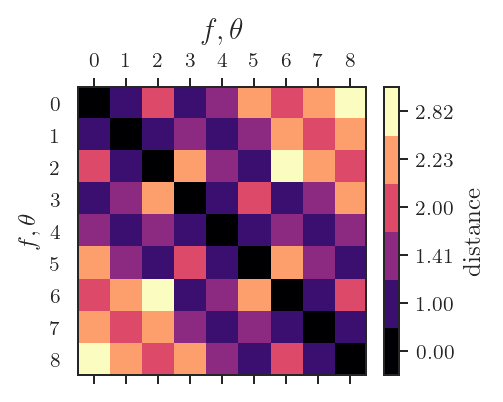
\includegraphics[width=\textwidth]{ground_distance_matrix_euclidean}	
		\caption{Euclidean}
        \label{fig:ground_distance_matrix_euclidean}
	\end{subfigure}
	~ %add desired spacing between images, e. g. ~, \quad, \qquad, \hfill etc. 
    %(or a blank line to force the subfigure onto a new line)
    \begin{subfigure}[b]{0.47\textwidth}
		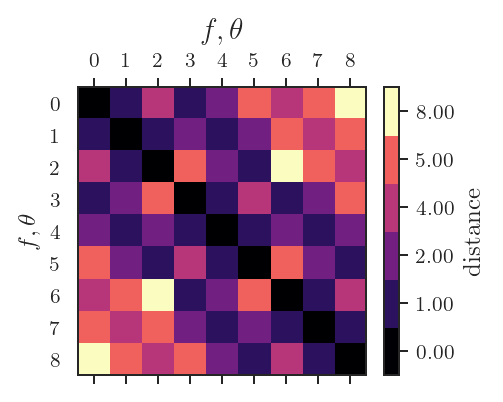
\includegraphics[width=\textwidth]{ground_distance_matrix_sqeuclidean}	
		\caption{Squared euclidean}
        \label{fig:ground_distance_matrix_sqeuclidean}
	\end{subfigure} \\[2ex]
    
    \begin{subfigure}[b]{0.47\textwidth}
		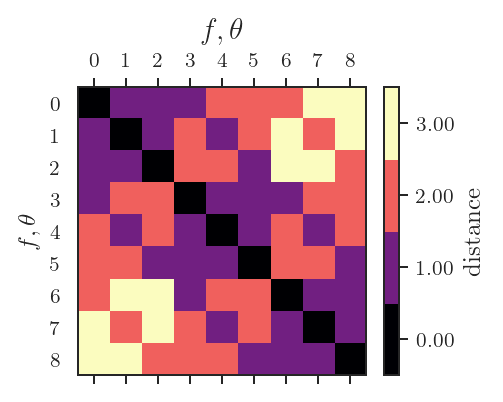
\includegraphics[width=\textwidth]{ground_distance_matrix_lin_polar}	
		\caption{Linear-polar}
        \label{fig:ground_distance_matrix_lin_polar}
	\end{subfigure}  
	~ %add desired spacing between images, e. g. ~, \quad, \qquad, \hfill etc. 
    %(or a blnk line to force the subfigure onto a new line)
	\begin{subfigure}[b]{0.47\textwidth}
		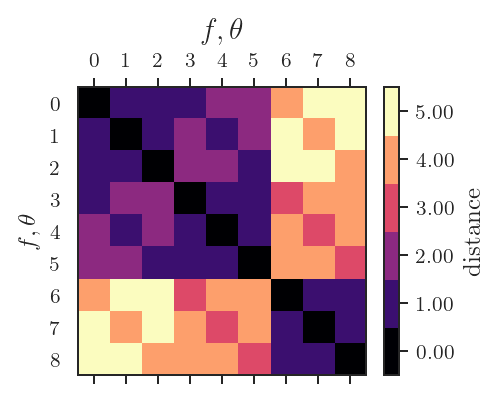
\includegraphics[width=\textwidth]{ground_distance_matrix_log_polar}	
		\caption{Log-polar}
        \label{fig:ground_distance_matrix_log_polar}
	\end{subfigure}  
	   
   \caption{Visualizations of cost matrix of EMD.}
   \label{fig:EMD_ground_distance_matrix}
\end{figure}


\section{Comparative Analysis of Similarity Measures}\label{sec:comparison}

\subsection{One-Dimensional Case Study}\label{subsec:1d_case}
To compare the measures described in section \ref{sec:measures} in the simplest scenario, we use a set of one-dimensional synthetic distributions. We create a source distribution and a series of target distributions (see Fig.\ \ref{fig:source_target_dist}). Both source and target distributions have 1000 samples and are random normal distributions. The unique difference between them is that the mean of each target distribution ($\mu$) is increasing five units concerning the previous distribution. The first target distribution is indiscernible from the source distribution.

\begin{figure}[ht] 
	\centering
	\begin{subfigure}[b]{0.45\textwidth}
		\centering
		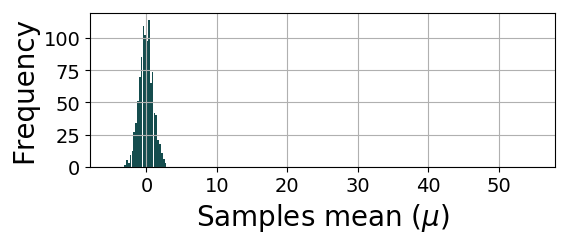
\includegraphics[width=\textwidth]{source_distribution}	
		\label{fig:source_distribution}
	\end{subfigure}
	~ %add desired spacing between images, e. g. ~, \quad, \qquad, \hfill etc. 
	%(or a blank line to force the subfigure onto a new line)
	\begin{subfigure}[b]{0.45\textwidth}
		\centering
		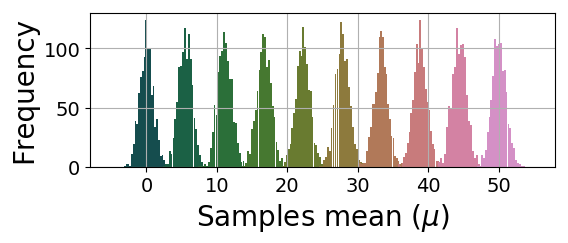
\includegraphics[width=\textwidth]{target_distributions}	
		\label{fig:targert_distributions}
	\end{subfigure}

  \caption{Source and target synthetic distributions.}
  \label{fig:source_target_dist}
\end{figure}


\begin{figure}[!ht]
    \centering
    \begin{subfigure}[b]{0.3\textwidth}
		\centering
		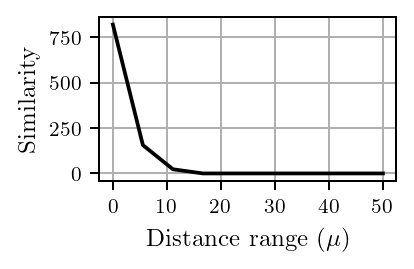
\includegraphics[width=\textwidth]{Inter_dist}	
		\caption{Histogram intersection}
        \label{fig:inter_dist}
	\end{subfigure}
	~ %add desired spacing between images, e. g. ~, \quad, \qquad, \hfill etc. 
    %(or a blank line to force the subfigure onto a new line)
    \begin{subfigure}[b]{0.3\textwidth}
		\centering
		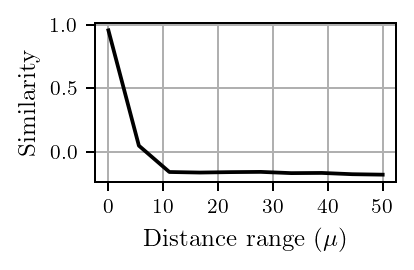
\includegraphics[width=\textwidth]{Corr_dist}	
		\caption{Histogram correlation}
        \label{fig:corr_dist}
	\end{subfigure}
    ~ %add desired spacing between images, e. g. ~, \quad, \qquad, \hfill etc. 
    %(or a blnk line to force the subfigure onto a new line)
    \begin{subfigure}[b]{0.3\textwidth}
		\centering
		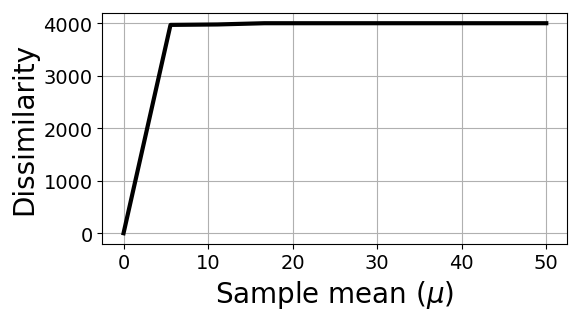
\includegraphics[width=\textwidth]{Chi2_dist}	
		\caption{$\chi^2$ Statistic}
        \label{fig:chi_square}
	\end{subfigure}  \\[2ex]
	
	
	\begin{subfigure}[b]{0.3\textwidth}
		\centering
		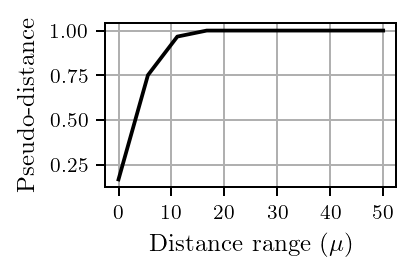
\includegraphics[width=\textwidth]{Bhatt_dist}	
		\caption{Bhattacharyya}
        \label{fig:bhatt_dist}
	\end{subfigure}
	~ %add desired spacing between images, e. g. ~, \quad, \qquad, \hfill etc. 
    %(or a blank line to force the subfigure onto a new line)    
    \begin{subfigure}[b]{0.3\textwidth}
		\centering
		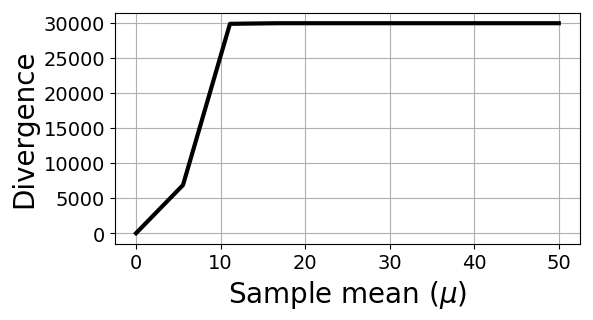
\includegraphics[width=\textwidth]{KL_dist}	
		\caption{Kullback-Leibler}
        \label{fig:kl_div}
	\end{subfigure}
    ~ %add desired spacing between images, e. g. ~, \quad, \qquad, \hfill etc. 
    %(or a blank line to force the subfigure onto a new line)
    \begin{subfigure}[b]{0.3\textwidth}
		\centering
		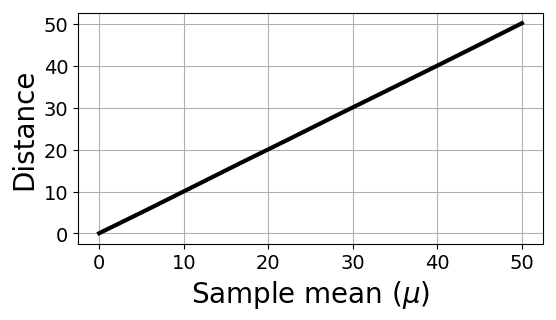
\includegraphics[width=\textwidth]{EMD_dist}	
		\caption{EMD}
        \label{fig:emd}
	\end{subfigure}
   
   \caption{Distances between the source and target distributions.}
   \label{fig:distances}
\end{figure}

Since the distributions' mean value increases linearly, we expect that the similarity measure has an equivalent response, i.e., that the similarity decreases when the difference of the source and target means increases. In Fig.\ \ref{fig:distances}, we can see the response of the bin-to-bin measures and the EMD. Among the bin-to-bin measures, those that give a coefficient of dissimilarity ($\chi^2$ statistic, Bhattacharyya pseudo-distance, and K-L divergence) rapidly saturate and stick to a maximum value; while for those that give a coefficient of similarity (histogram correlation and intersection), their value falls rapidly to zero. We can interpret these behaviors as follows. When the bins $p_i$, $q_i$ do not have any mass in common, the bin-to-bin measures fail to consider the mutual distance of the bins. They could consider that the distributions are precisely at the same distance (there is no difference between them), or that the distributions are entirely dissimilar. The only measure that presents a convenient behavior with the increasing difference of the means is the EMD. This is due to taking into account the \textit{ground distance} $\mathbf{C}$ of the matching bins (see above, Eq. \eqref{eq:emd}). One can argue that for applications like image retrieval finding the most similar distribution is sufficient to find the alike image or texture, whereas the ordering on the other is irrelevant. In the following experiment, we show that this intuition is incorrect and that even in an overly simple case, the bin-to-bin measures are not the best choice.
 
\subsection{Image Retrieval Systems}
We develop two image retrieval systems as a second comparison test, the first based on color information and the second based on texture information. For the classifiers, we use different databases. The first one contains 24 different color images of superhero toys\footnote{CC super hero's images courtesy of Christopher Chong on Flickr.}. It has 12 classes with two samples per class. The first two rows in Fig.\ \ref{fig:databases} show some examples of the superhero toys and their variations (change of the angle of the toy or the addition of accessories). The second database \citep{Kylberg:Dataset:2011} comprises images belonging to different surfaces and materials (see the last two rows in Fig.\ \ref{fig:databases}). The database contains 28 different classes; it contains different patches per class. 

\begin{figure}[!ht]
	\centering
	\begin{subfigure}[b]{0.12\textwidth}
		\centering
		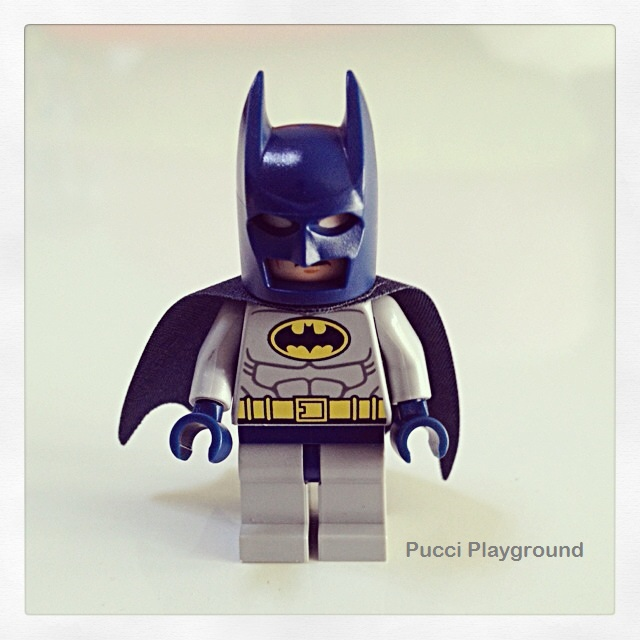
\includegraphics[width=\textwidth]{batman1_model}	
	\end{subfigure}
	~ %add desired spacing between images, e. g. ~, \quad, \qquad, \hfill etc. 
    %(or a blank line to force the subfigure onto a new line)
    \begin{subfigure}[b]{0.12\textwidth}
		\centering
		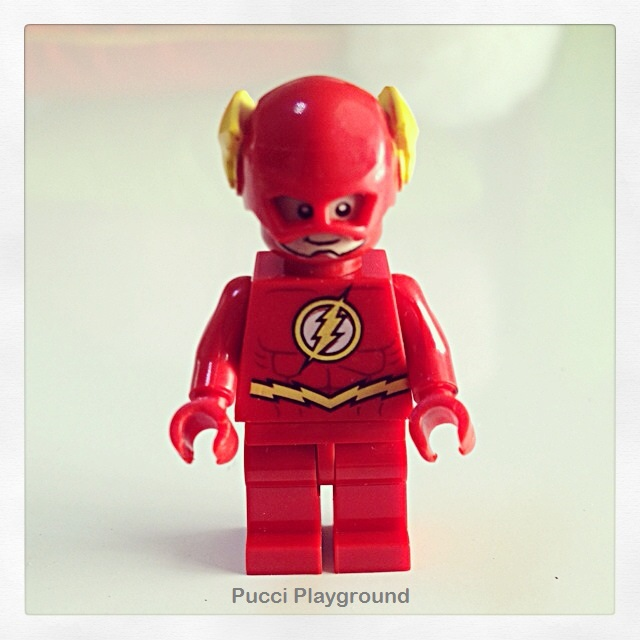
\includegraphics[width=\textwidth]{flash_model}	
	\end{subfigure}
    ~ %add desired spacing between images, e. g. ~, \quad, \qquad, \hfill etc. 
    %(or a blank line to force the subfigure onto a new line)
    \begin{subfigure}[b]{0.12\textwidth}
		\centering
		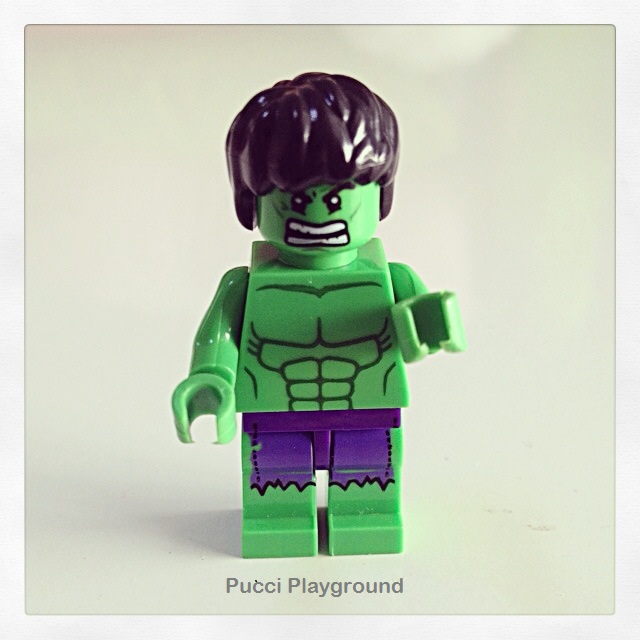
\includegraphics[width=\textwidth]{hulk_model}	
	\end{subfigure}
	~ %add desired spacing between images, e. g. ~, \quad, \qquad, \hfill etc. 
    %(or a blank line to force the subfigure onto a new line)
    \begin{subfigure}[b]{0.12\textwidth}
		\centering
		
\includegraphics[width=\textwidth]{wonderwoman_model}	
	\end{subfigure}
    ~ %add desired spacing between images, e. g. ~, \quad, \qquad, \hfill etc. 
    %(or a blank line to force the subfigure onto a new line)
    \begin{subfigure}[b]{0.12\textwidth}
		\centering
		
\includegraphics[width=\textwidth]{wolverine_model}	
	\end{subfigure}
    ~ %add desired spacing between images, e. g. ~, \quad, \qquad, \hfill etc. 
    %(or a blank line to force the subfigure onto a new line)
    \begin{subfigure}[b]{0.12\textwidth}
		\centering
		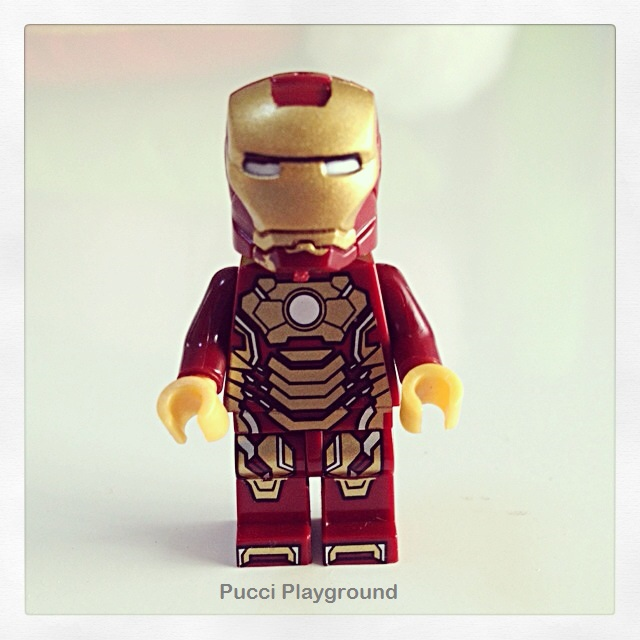
\includegraphics[width=\textwidth]{ironman_model}	
	\end{subfigure}
    ~ %add desired spacing between images, e. g. ~, \quad, \qquad, \hfill etc. 
    %(or a blank line to force the subfigure onto a new line)
    \begin{subfigure}[b]{0.12\textwidth}
		\centering
		
\includegraphics[width=\textwidth]{thor_model}	
	\end{subfigure} \\[2ex]
    
        
    \begin{subfigure}[b]{0.12\textwidth}
		\centering
		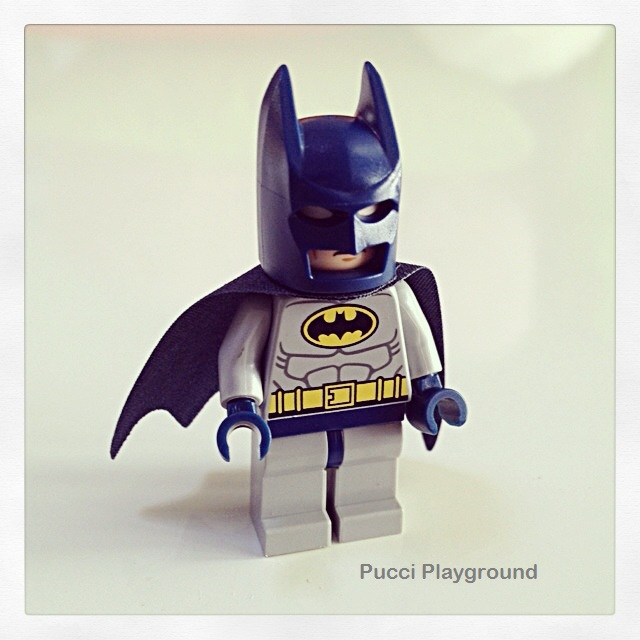
\includegraphics[width=\textwidth]{batman1}	
	\end{subfigure}
	~ %add desired spacing between images, e. g. ~, \quad, \qquad, \hfill etc. 
    %(or a blank line to force the subfigure onto a new line)
    \begin{subfigure}[b]{0.12\textwidth}
		\centering
		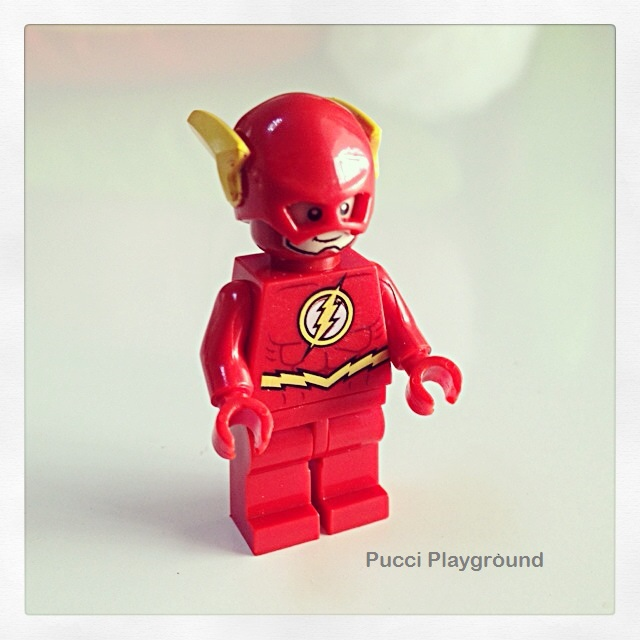
\includegraphics[width=\textwidth]{flash}	
	\end{subfigure}
    ~ %add desired spacing between images, e. g. ~, \quad, \qquad, \hfill etc. 
    %(or a blank line to force the subfigure onto a new line)
    \begin{subfigure}[b]{0.12\textwidth}
		\centering
		
\includegraphics[width=\textwidth]{hulk}	
	\end{subfigure}
	~ %add desired spacing between images, e. g. ~, \quad, \qquad, \hfill etc. 
    %(or a blank line to force the subfigure onto a new line)
    \begin{subfigure}[b]{0.12\textwidth}
		\centering
		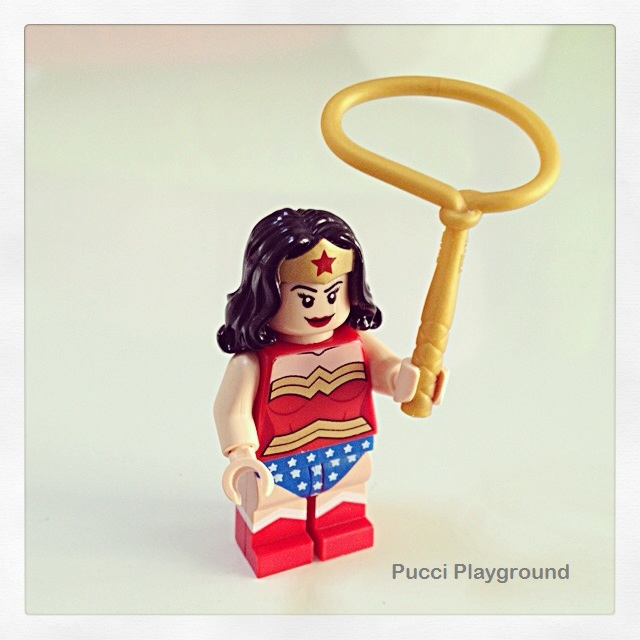
\includegraphics[width=\textwidth]{wonderwoman}	
	\end{subfigure}
    ~ %add desired spacing between images, e. g. ~, \quad, \qquad, \hfill etc. 
    %(or a blank line to force the subfigure onto a new line)
    \begin{subfigure}[b]{0.12\textwidth}
		\centering
		
\includegraphics[width=\textwidth]{wolverine}	
	\end{subfigure}
    ~ %add desired spacing between images, e. g. ~, \quad, \qquad, \hfill etc. 
    %(or a blank line to force the subfigure onto a new line)
    \begin{subfigure}[b]{0.12\textwidth}
		\centering
		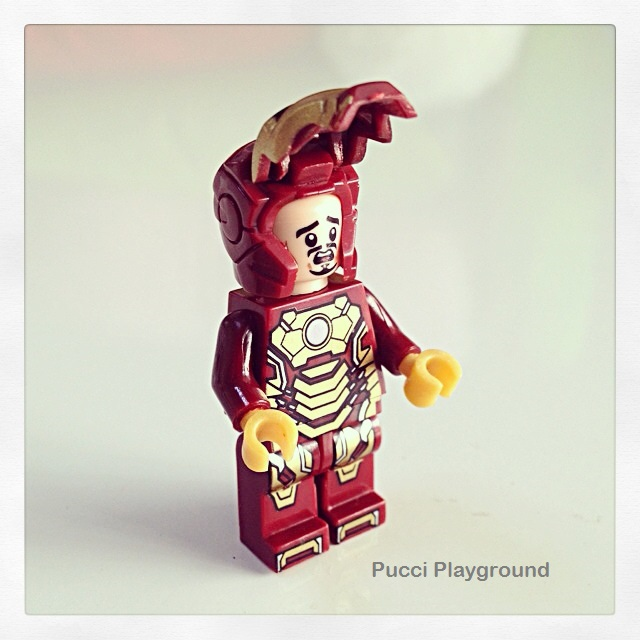
\includegraphics[width=\textwidth]{ironman_b}	
	\end{subfigure}
    ~ %add desired spacing between images, e. g. ~, \quad, \qquad, \hfill etc. 
    %(or a blank line to force the subfigure onto a new line)
    \begin{subfigure}[b]{0.12\textwidth}
		\centering
		
\includegraphics[width=\textwidth]{thor}	
	\end{subfigure} \\[2ex]
    
    
    \begin{subfigure}[b]{0.12\textwidth}
		\centering
		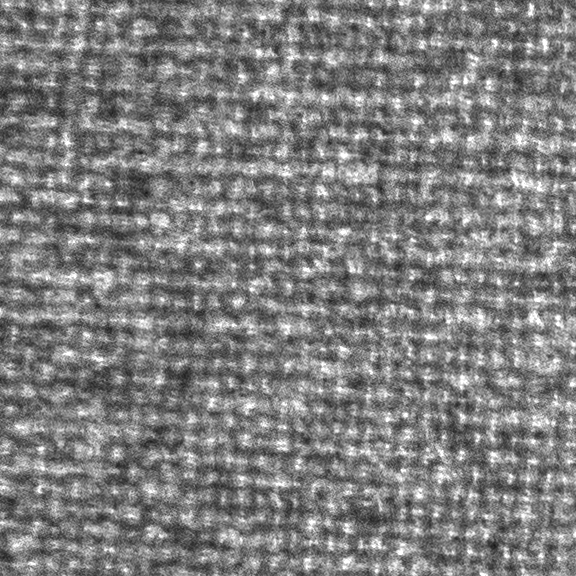
\includegraphics[width=\textwidth]{blanket1}	
	\end{subfigure}
	~ %add desired spacing between images, e. g. ~, \quad, \qquad, \hfill etc. 
    %(or a blank line to force the subfigure onto a new line)
    \begin{subfigure}[b]{0.12\textwidth}
		\centering
		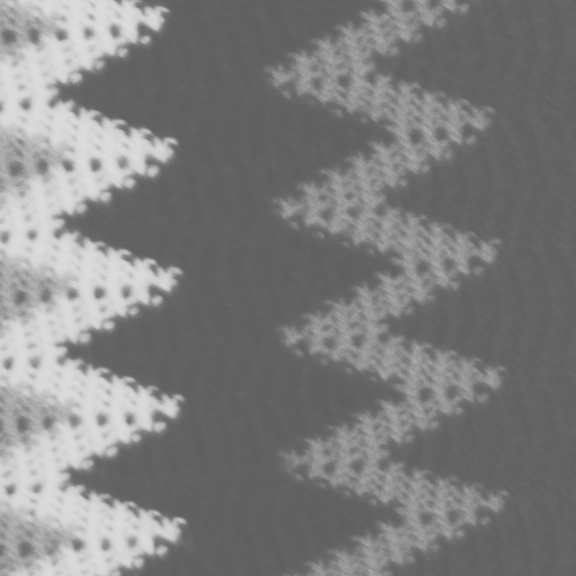
\includegraphics[width=\textwidth]{blanket2}	
	\end{subfigure}
    ~ %add desired spacing between images, e. g. ~, \quad, \qquad, \hfill etc. 
    %(or a blank line to force the subfigure onto a new line)
    \begin{subfigure}[b]{0.12\textwidth}
		\centering
		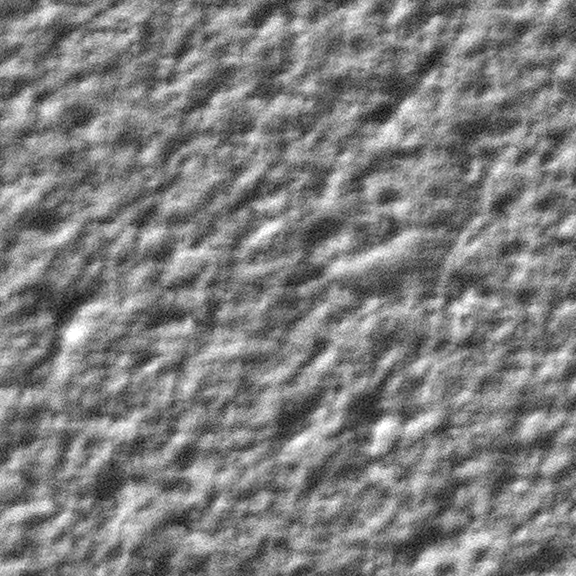
\includegraphics[width=\textwidth]{ceiling1}	
	\end{subfigure}
	~ %add desired spacing between images, e. g. ~, \quad, \qquad, \hfill etc. 
    %(or a blank line to force the subfigure onto a new line)
    \begin{subfigure}[b]{0.12\textwidth}
		\centering
		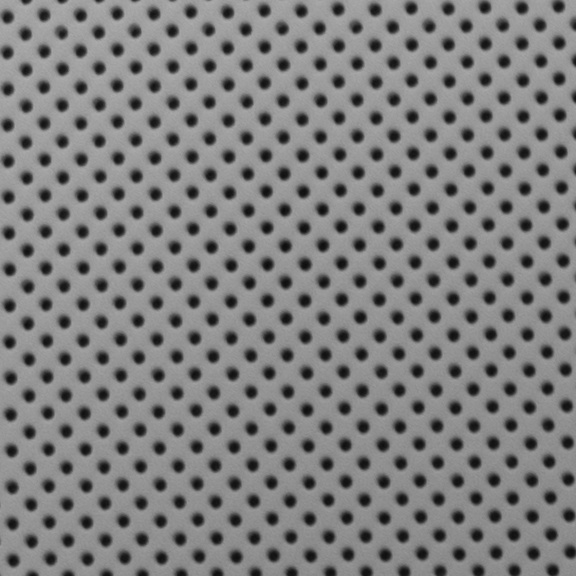
\includegraphics[width=\textwidth]{ceiling2}	
	\end{subfigure}
    ~ %add desired spacing between images, e. g. ~, \quad, \qquad, \hfill etc. 
    %(or a blank line to force the subfigure onto a new line)
    \begin{subfigure}[b]{0.12\textwidth}
		\centering
		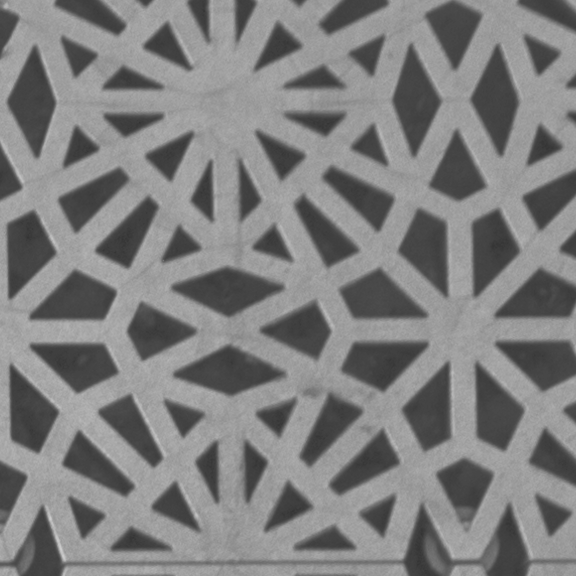
\includegraphics[width=\textwidth]{floor1}	
	\end{subfigure}
    ~ %add desired spacing between images, e. g. ~, \quad, \qquad, \hfill etc. 
    %(or a blank line to force the subfigure onto a new line)
    \begin{subfigure}[b]{0.12\textwidth}
		\centering
		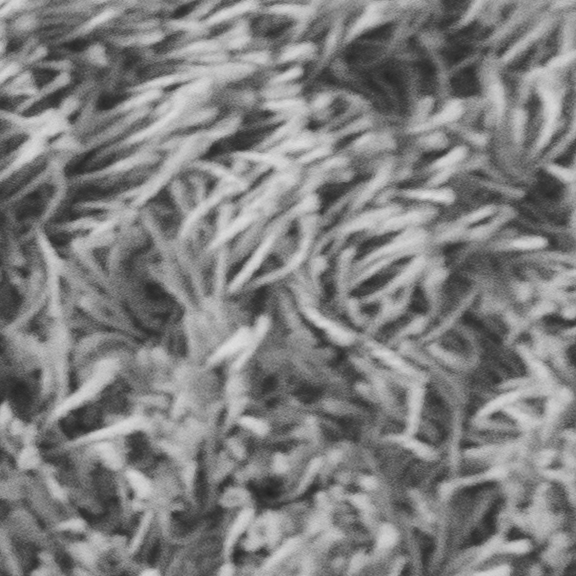
\includegraphics[width=\textwidth]{rug}	
	\end{subfigure}
    ~ %add desired spacing between images, e. g. ~, \quad, \qquad, \hfill etc. 
    %(or a blank line to force the subfigure onto a new line)
    \begin{subfigure}[b]{0.12\textwidth}
		\centering
		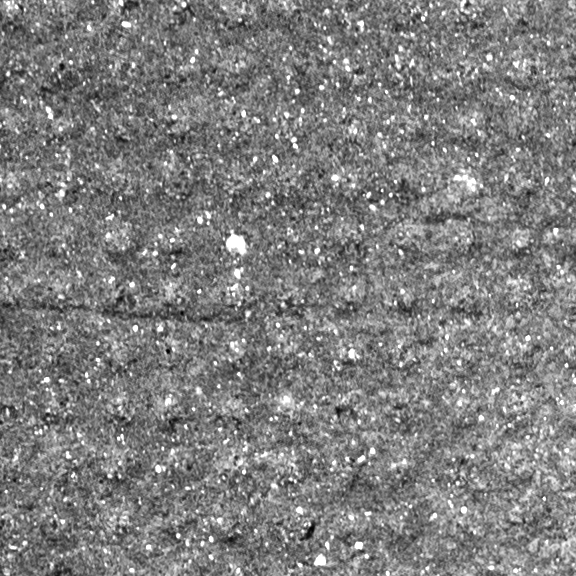
\includegraphics[width=\textwidth]{stoneslab}	
	\end{subfigure} \\[2ex]
    
        
    \begin{subfigure}[b]{0.12\textwidth}
		\centering
		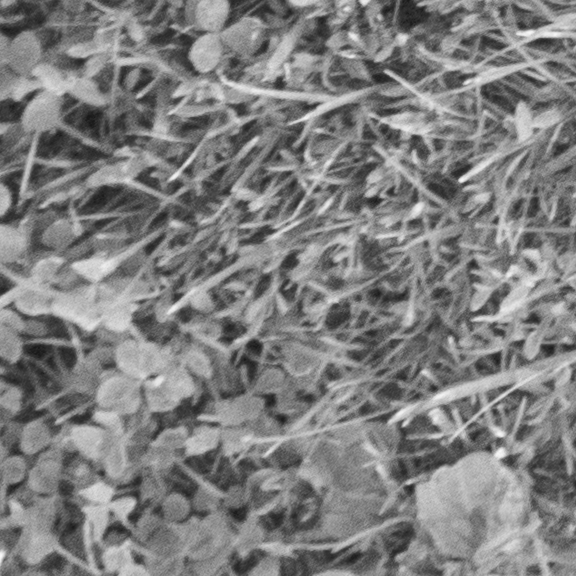
\includegraphics[width=\textwidth]{grass}	
	\end{subfigure}
	~ %add desired spacing between images, e. g. ~, \quad, \qquad, \hfill etc. 
    %(or a blank line to force the subfigure onto a new line)
    \begin{subfigure}[b]{0.12\textwidth}
		\centering
		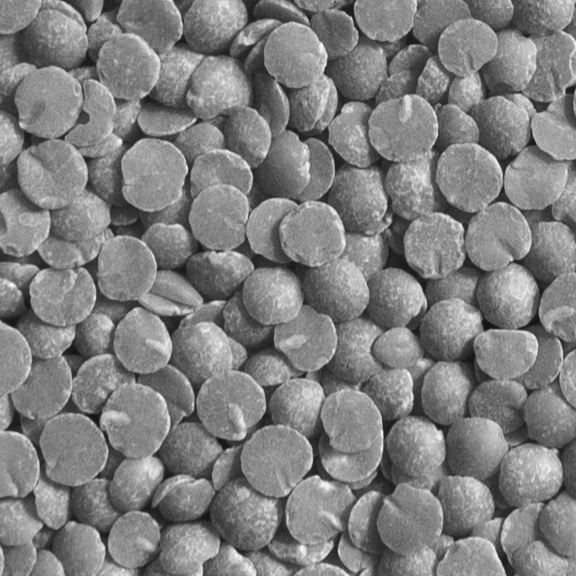
\includegraphics[width=\textwidth]{lentils}	
	\end{subfigure}
    ~ %add desired spacing between images, e. g. ~, \quad, \qquad, \hfill etc. 
    %(or a blank line to force the subfigure onto a new line)
    \begin{subfigure}[b]{0.12\textwidth}
		\centering
		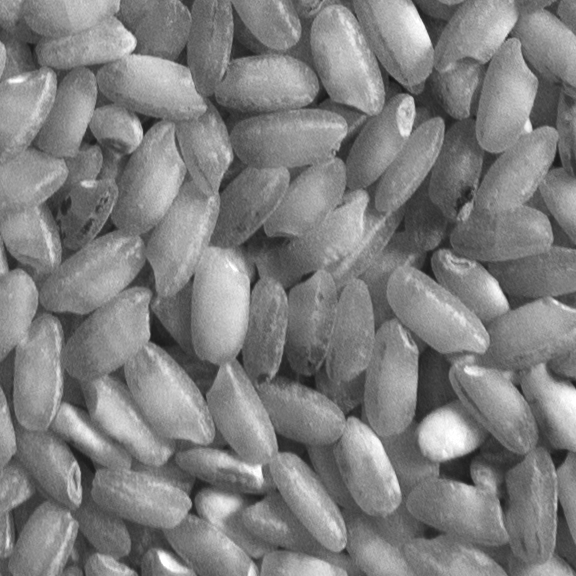
\includegraphics[width=\textwidth]{rice2}	
	\end{subfigure}
	~ %add desired spacing between images, e. g. ~, \quad, \qquad, \hfill etc. 
    %(or a blank line to force the subfigure onto a new line)
    \begin{subfigure}[b]{0.12\textwidth}
		\centering
		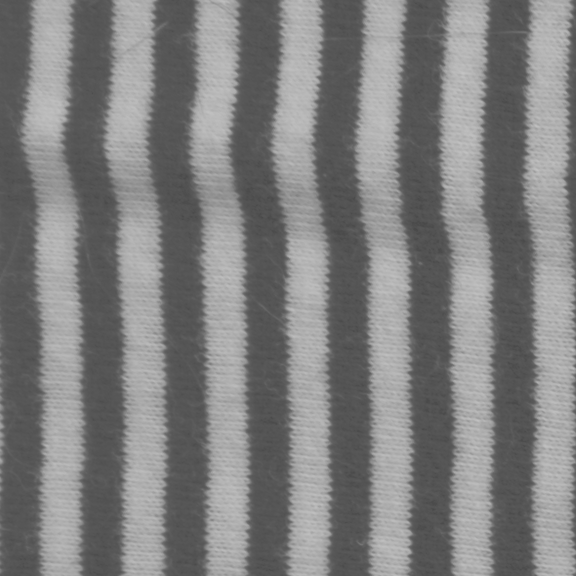
\includegraphics[width=\textwidth]{scarf2}	
	\end{subfigure}
    ~ %add desired spacing between images, e. g. ~, \quad, \qquad, \hfill etc. 
    %(or a blank line to force the subfigure onto a new line)
    \begin{subfigure}[b]{0.12\textwidth}
		\centering
		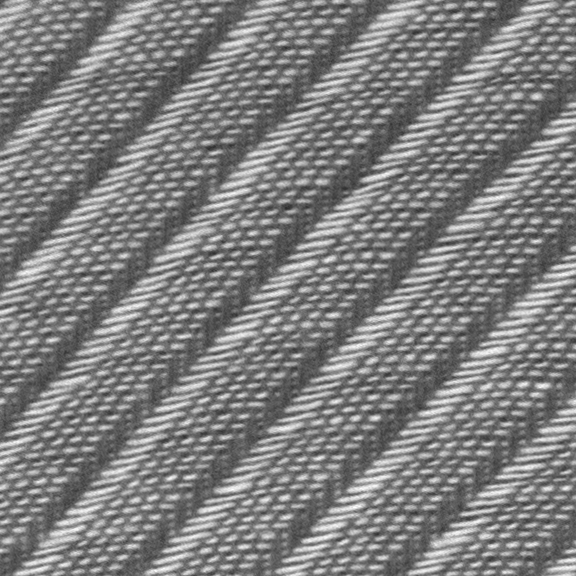
\includegraphics[width=\textwidth]{screen}	
	\end{subfigure}
    ~ %add desired spacing between images, e. g. ~, \quad, \qquad, \hfill etc. 
    %(or a blank line to force the subfigure onto a new line)
    \begin{subfigure}[b]{0.12\textwidth}
		\centering
		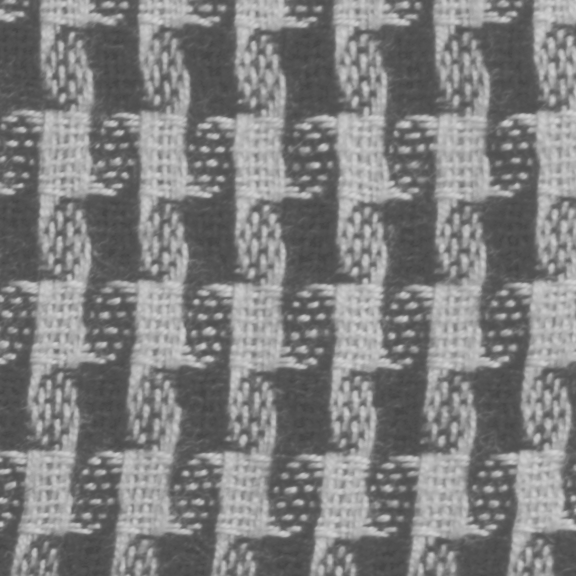
\includegraphics[width=\textwidth]{scarf1}	
	\end{subfigure}
    ~ %add desired spacing between images, e. g. ~, \quad, \qquad, \hfill etc. 
    %(or a blank line to force the subfigure onto a new line)
    \begin{subfigure}[b]{0.12\textwidth}
		\centering
		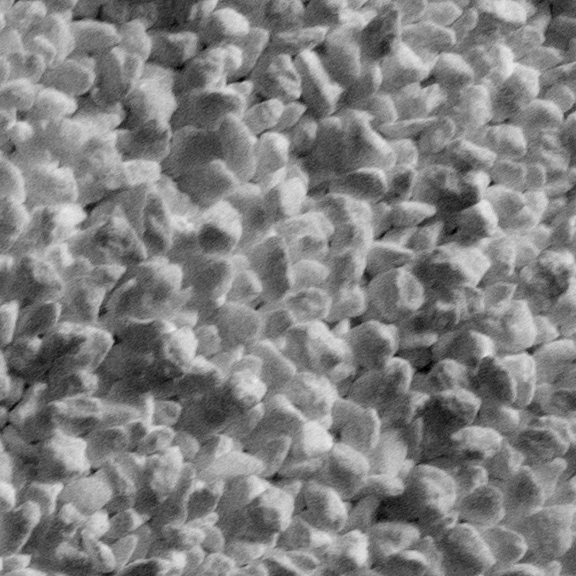
\includegraphics[width=\textwidth]{pearlsugar}	
	\end{subfigure}
		
    \caption{Some samples from the color and texture databases.}
    \label{fig:databases}
\end{figure}

We compare the performance of six out of the eight measures described in section \ref{sec:measures} in the following way. First, we divide the database samples into \textit{model images} and \textit{query images}; each class only has one model and one query image. We select an image from the query set and compare its color/texture distribution (source distribution) with all model images' color/texture distribution (target distributions). Then, we order the images from the most similar to the most dissimilar image. We repeat this process for all the images in the query set\footnote{The image classification systems (color-based and texture-based) and the datasets used for this chapter are available at \url{https://github.com/CVMethods/image_clasifier.git}}.
 
\textbf{Image color distribution.} We use 3-d histograms to represent the distribution of color pixels. Since the superhero images are very simple and do not present significant challenges, i.e., the images possess a very distinctive color palette and do not present textures or important changes in lighting, any similarity measure should be sufficient to perform the image retrieval. However, image retrieval systems are sensitive to the representation and quantification of the color image pixels. We show this effect by varying the color space and the color quantization level in the image classifier. We represent the images in the RGB, HSL, and LAB color spaces for the color space. We represent the color space in histograms of 8, 16, and 32 bins per channel for the color quantization level.

\textbf{Image texture distribution.} We use a family of Gabor filters as texture descriptors to obtain a distribution (2-d histograms) that models the images' texture. This type of filter models the human visual cortex's behavior \citep{Daugman:TASSP:1988}, so they are very useful in computer vision applications to represent textures \citep{Lee:PAMI:1996}. The mother wavelet
\begin{eqnarray}
 g(x,y,\omega,\theta) = \frac{\omega^2}{4\pi\kappa^2} \mathsf{e}^{-\frac{\omega^2}{8\kappa^2}\left(4\hat{x}^2 + \hat{y}^2\right)} \cdot [\mathsf{e}^{i \kappa \hat{x}} -\mathsf{e}^ {\frac{\kappa ^ 2}{2}} ]  \label{eq:gabor_filters}
\end{eqnarray}
represents the family of Gabor descriptors, where $\hat{x} = x \cos \theta +  y \sin \theta$ and $\hat{y} = -x\sin \theta + y \cos \theta$ . The 2-d texture histograms are a function of the Gabor responses' energies according to the frequency $\omega$, the orientation $\theta$ and the constant $\kappa$ in the Gabor wavelet. The 2-d texture histograms are a function of the Gabor responses' energies according to the frequency  $\kappa \approx \pi$ and six bins means that there are six different frequencies to a bandwidth of one octave and six different orientations. The energy of a Gabor response is given by
\begin{eqnarray} 
 E_{\omega,\theta} = \sum\nolimits_{x, y}|W_{x,y,\omega,\theta}|^2, \label{eq:g_energy}
\end{eqnarray}
where $W_{x,y,\omega,\theta}$ is the response of the convolution of a 2-d wavelet with frequency $\omega$ and orientation $\theta$ with an image. 

\subsubsection{Image Retrieval Systems Evaluation} \label{subsubsec:evaluation}

We create a comparison benchmark for the six similarity measures. First, we normalize the distances given by the different methods between $0$ and $1$, where a value close to $0$ means the most similar distribution to the source distribution and $1$ the most dissimilar. Then we transform the normalized distances into probabilities using a softmax function $SM(\mathbf{d}) = \frac{\mathsf{e}^{\mathbf{d}}}{\sum_{i}\mathsf{e}^{d_i}}$. The vector $\mathbf{d}=\{d_i\}$, $\forall i=\{1, \ldots, M\}$, represents the distances between the query image to the $M$ images in the database. Considering the softmax function of the distances vector as a classification probability $SM(\mathbf{d})=\mathbf{\hat{y}}$,  we compute the cross-entropy \citep{Bishop:BOOK:2006} considering the classification ground truth $\mathbf{y}$ such as, 
\begin{eqnarray}
H(\mathbf{y}, \mathbf{\hat{y}}) = - \sum\nolimits_{i}{y_i}\log \hat{y}_i
\label{eq:cross-entropy}
\end{eqnarray}
where $y_i$ is the ground truth probability vector, and $\hat{y}_i$ the probability vector of the prediction.


We can interpret the cross-entropy value as the image classifier's confidence level for some given metric, feature space (color or texture), and histogram size. When this value is very close to zero, it indicates a perfect classification of the query image. In Fig.\ \ref{fig:cross_entropy}, we note the superiority of the EMD over the other measures in both color and texture-based classifiers.

\begin{figure}[ht]
    \centering
    \begin{subfigure}[b]{0.48\textwidth}
		\centering
		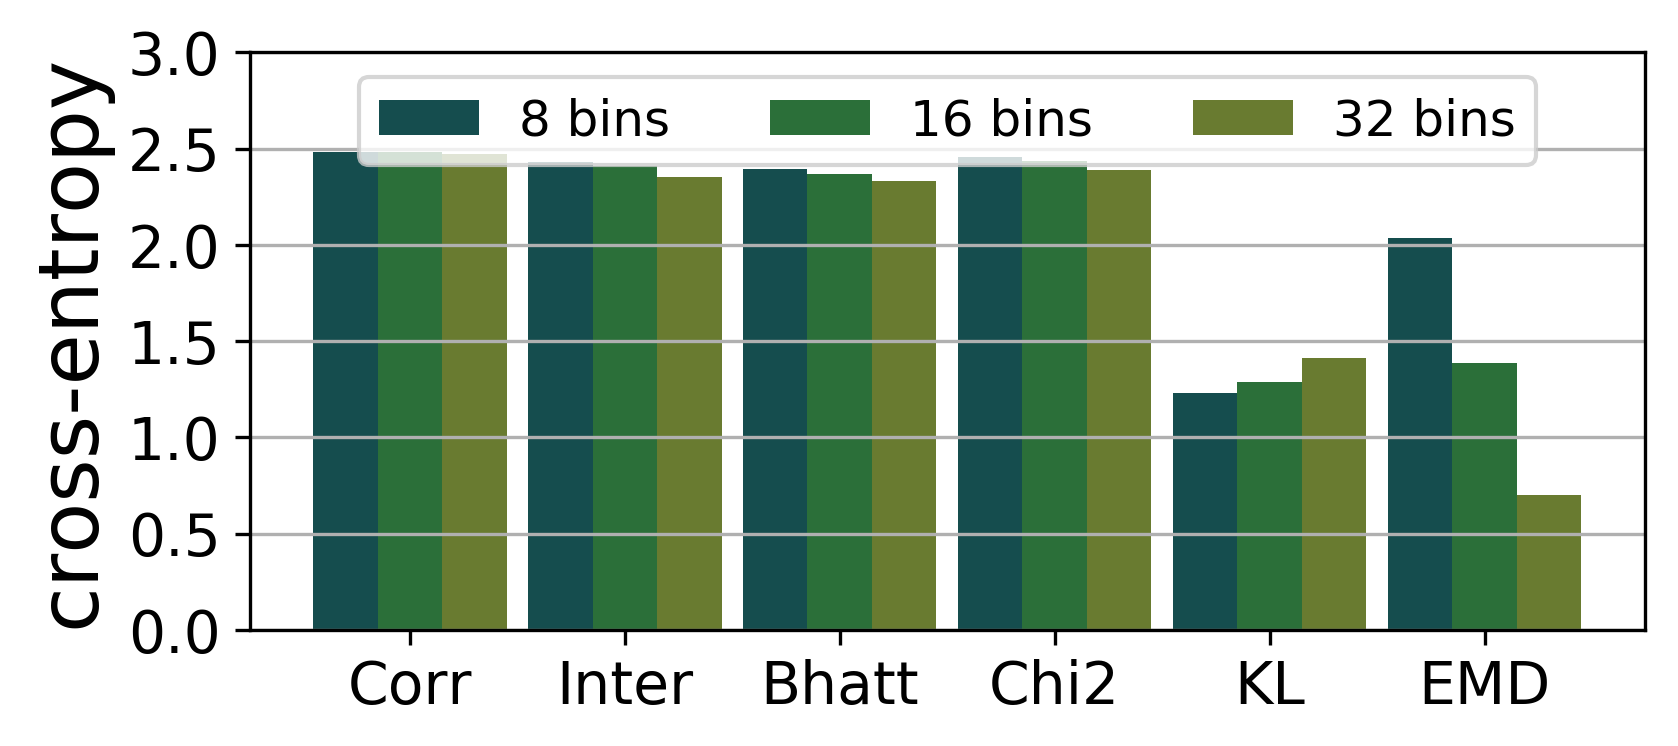
\includegraphics[width=\textwidth]{log_loss_rgb}	
		\caption{RGB color space}
	\end{subfigure}
    ~ %add desired spacing between images, e. g. ~, \quad, \qquad, \hfill etc. 
    %(or a blank line to force the subfigure onto a new line)
    \begin{subfigure}[b]{0.48\textwidth}
		\centering
		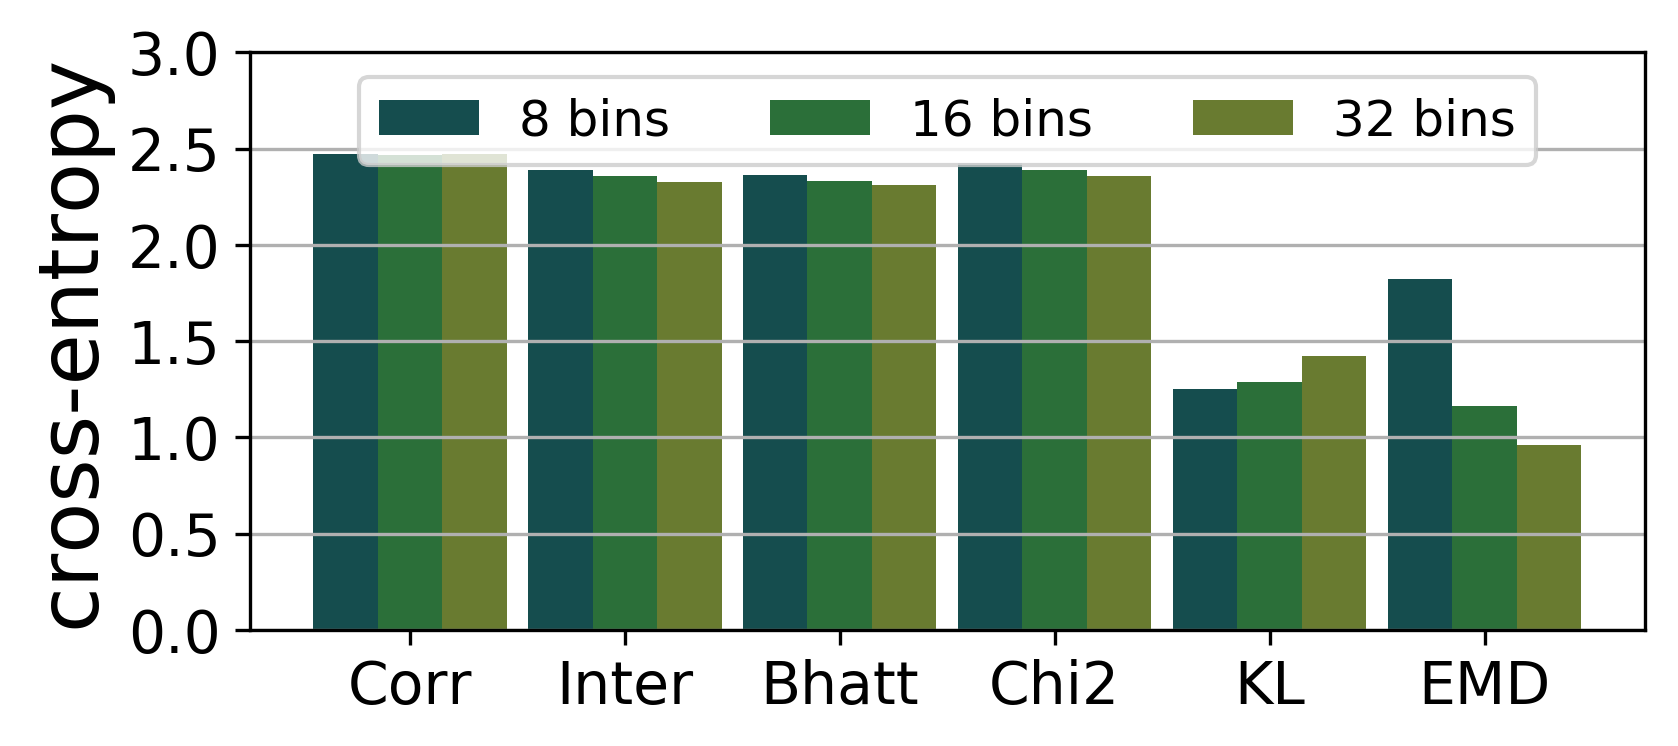
\includegraphics[width=\textwidth]{log_loss_hls}	
		\caption{HLS color space}
	\end{subfigure}\\[2ex]
	
	
    \begin{subfigure}[b]{0.48\textwidth}
		\centering
		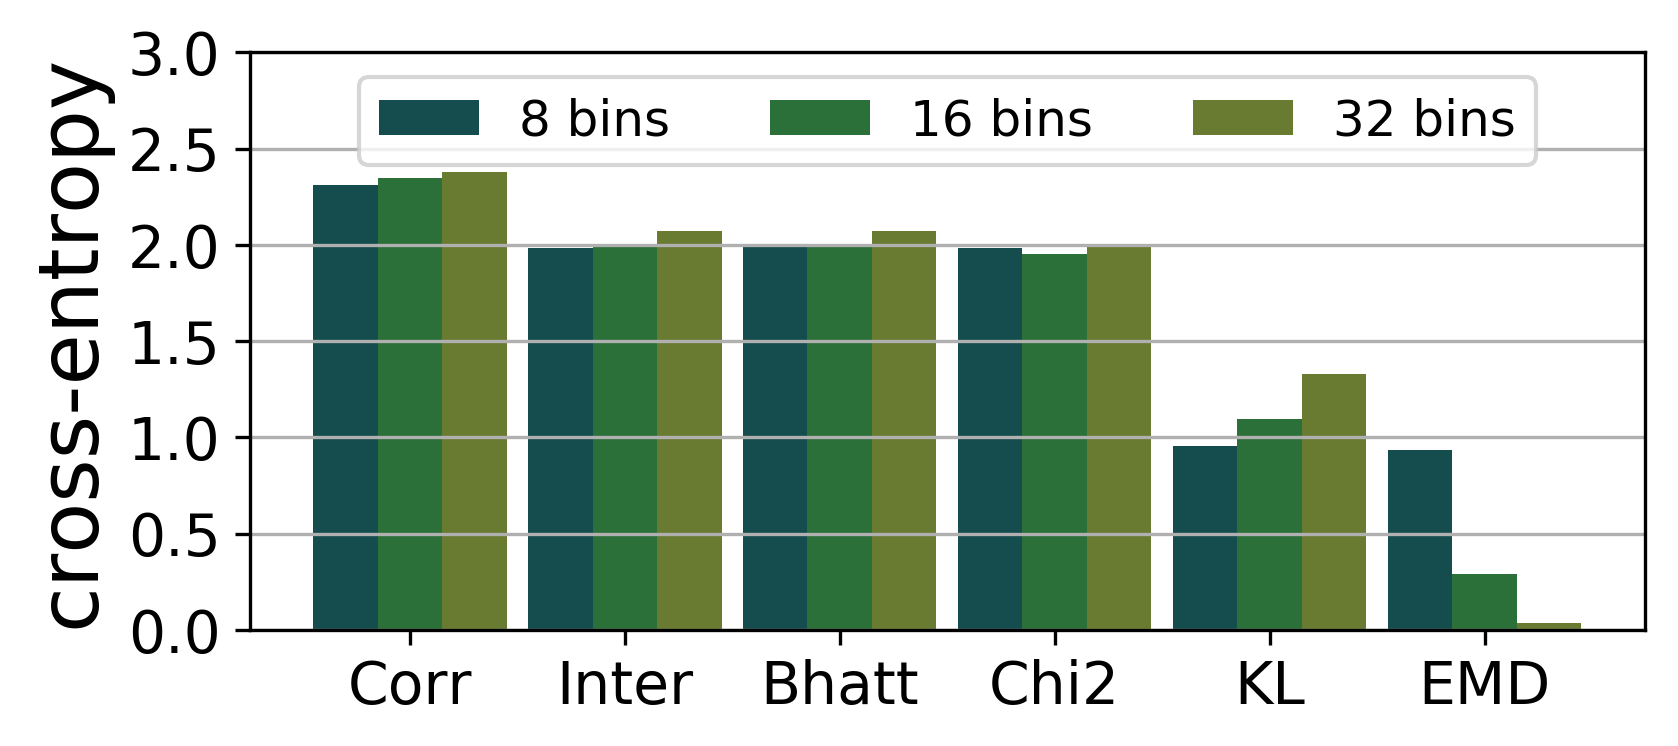
\includegraphics[width=\textwidth]{log_loss_lab}	
		\caption{LAB color space}
	\end{subfigure}   
    ~ %add desired spacing between images, e. g. ~, \quad, \qquad, \hfill etc. 
    %(or a blank line to force the subfigure onto a new line)
    \begin{subfigure}[b]{0.48\textwidth}
		\centering
		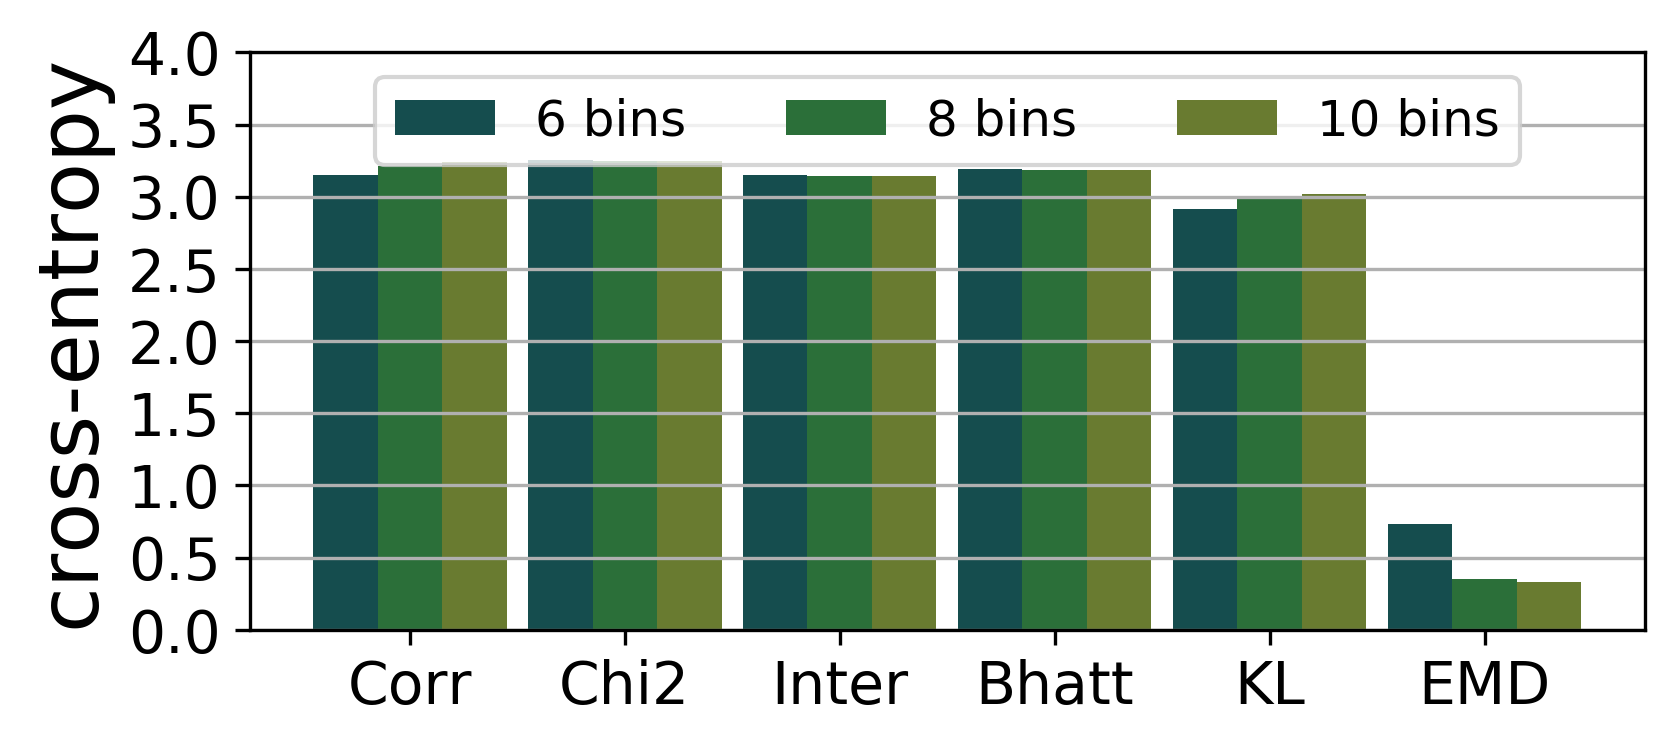
\includegraphics[width=\textwidth]{log_loss_texture}	
		\caption{Texture Gabor energy space (Eq. \eqref{eq:g_energy})}
	\end{subfigure}  
		
	\caption{Cross entropy value of image retrieval systems (color and texture) using different similarity measures (lower is better).}
	\label{fig:cross_entropy}
\end{figure}

With the image retrieval systems, we can highlight interesting aspects of the EMD and the use of bin-to-bin measures in the comparison of distributions. First, we see the importance of selecting the color space and the compression level of the feature space (histogram size). The effect of discretization in the bin-to-bin measures is counter-intuitive because the error increases slightly when the number of bins increases. The explanation could be a poorer intersection of mass distributions. In the case of EMD, increasing the number of bins improves the classification result. Besides, as we expected, in the color-based classifier, the calculation of the EMD using the LAB color space performs better than with the HLS or the RGB. This effect is because the LAB color space models the color human perception in the Euclidean space; therefore, the \textit{ground distance} between two colors is easily calculated with the $L_2$ norm. On the other hand, in the texture-based classifier, increasing the number of bins beyond eight bins does not improve the classification considerably. This behavior occurs because the histograms with eight frequencies and eight orientations represent sufficiently well the image textures.

\subsection{Texture Projection Quality Evaluation} \label{subsec:mds}

We use the multidimensional scaling (MDS) technique \citep{Kruskal:Psycho:1964} as the last evaluation test for the similarity measures on the texture dataset. The MDS allows to geometrically represent $n$ textures using a set of $n$ points $\{x_1, \ldots, x_n\}$ in a reduced Euclidean space $\mathbb{R}^{d}$ so that the distances between the points $\hat{d}_{ij} = ||x_i-x_j||_2$ correspond as much as possible to the values of dissimilarity $d_{ij}$ between the texture distributions. To evaluate the quality of the projection, we use the stress value proposed in \citep{Kruskal:Psycho:1964}.
\begin{eqnarray}
S= \sqrt{\frac{\sum_{ij}(\hat{d}_{ij}-d_{ij})^2}{\sum_{ij}\hat{d}_{ij}^2}}
\label{eq:stress}
\end{eqnarray}

The stress coefficient is a positive value that indicates how well the distances given by the measures are preserved in the new low-dimensional space, i.e., the lower the level of $S$, the better the representation of texture in a low-dimensional space (2-d in our case). Fig.\ \ref{fig:stress} shows how the lowest stress is obtained using the EMD. This result is because the MDS technique interprets the distances of the entrance towards distances in a low dimension space. Given that the EMD is the only measure that is a true metric, not only is the stress level low, but the visual projection is following the frequency $\omega$ and orientation $\theta$ used in the Gabor filters (Eq. \eqref{eq:gabor_filters}) that model the distribution of the textures (see Fig.\ \ref{fig:MDS_EMD}). %in the appendix \ref{ch:suplementary_material_retrieval_systems}

\begin{figure}[!ht]
    \centering
    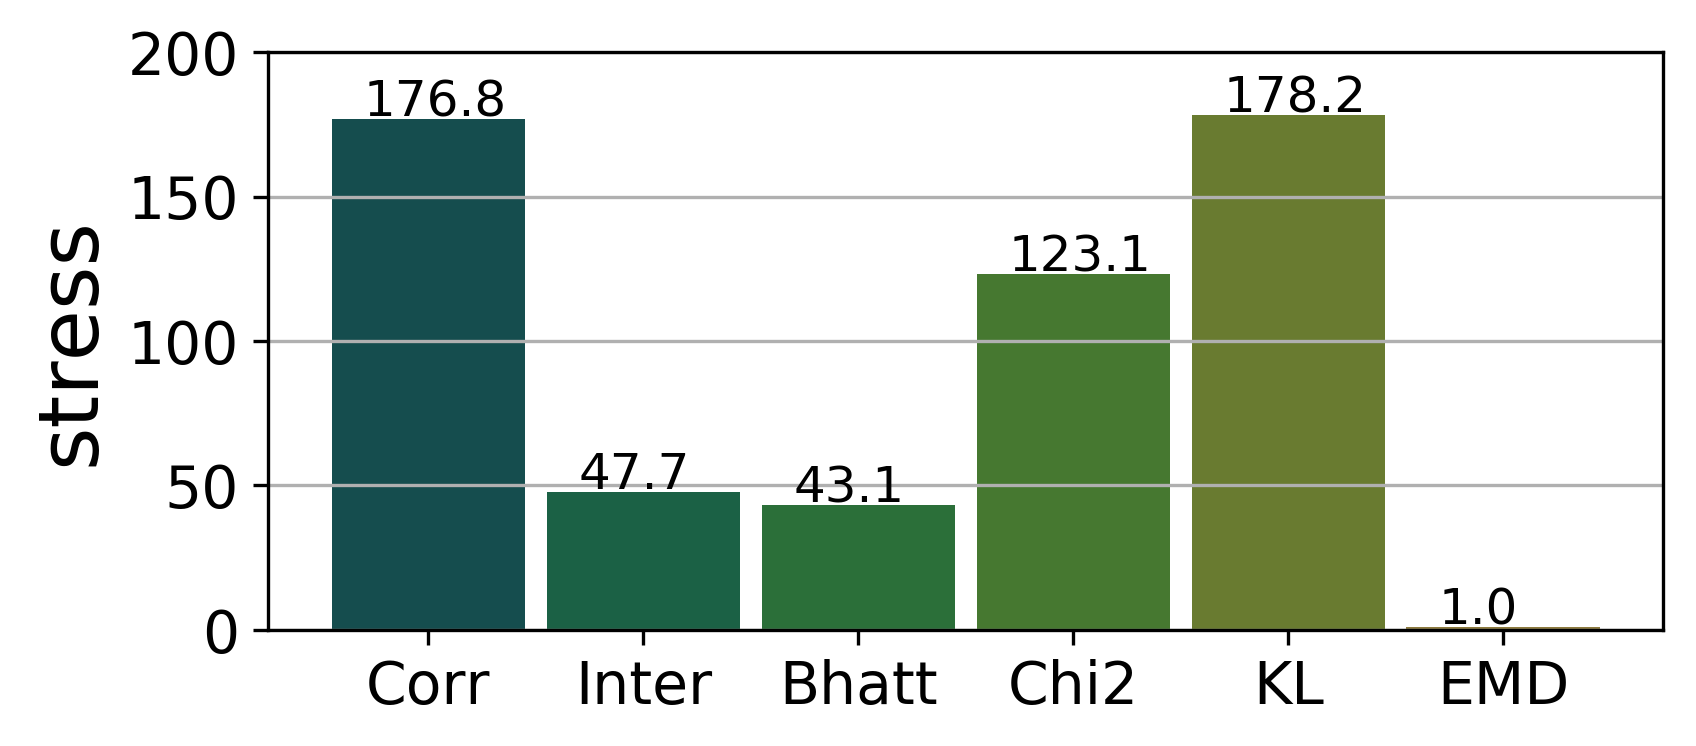
\includegraphics[width=0.45\textwidth]{stress}
 \caption{Stress value of the MDS projections using the six principal similarity measures.}
 \label{fig:stress}
\end{figure}

\subsection{Color and Texture Retrieved Images: Some Cases of Study}\label{ch:suplementary_material_retrieval_systems}

\subsubsection{Color-based Image Retrieval}\label{sec:sm_color:class}
The Figs.\ \ref{fig:wonderwoman_distances} and \ref{fig:superman_distances} present the result of the classification of the images of two superhero toys. The query image is displayed in the upper left. The rows of the image arrangement represent the different measurements used in the retrieval, while the columns show the most similar image from left to right in descending order. The numerical values of the distances are below each image; these values are not normalized, nor are they on the same scale. Notice that some values are sorted in decreasing whereas some others in increasing order. The various distances are increasing, the similarity measures (correlation, intersection) are decreasing.

The two examples here show how, under certain disturbances in color distribution, bin-to-bin measurements cannot identify the correct result. For the Wonderwoman toy, the fact that the query image has an extra accessory modifies the color signature of the image, while in the case of the superman toy, the color signature is very close to those toys that contain red and blue colors. These two images were obtained using the LAB color space and 32 bins for the pixels' color distribution.
\begin{figure}[!ht]
 \centering    
 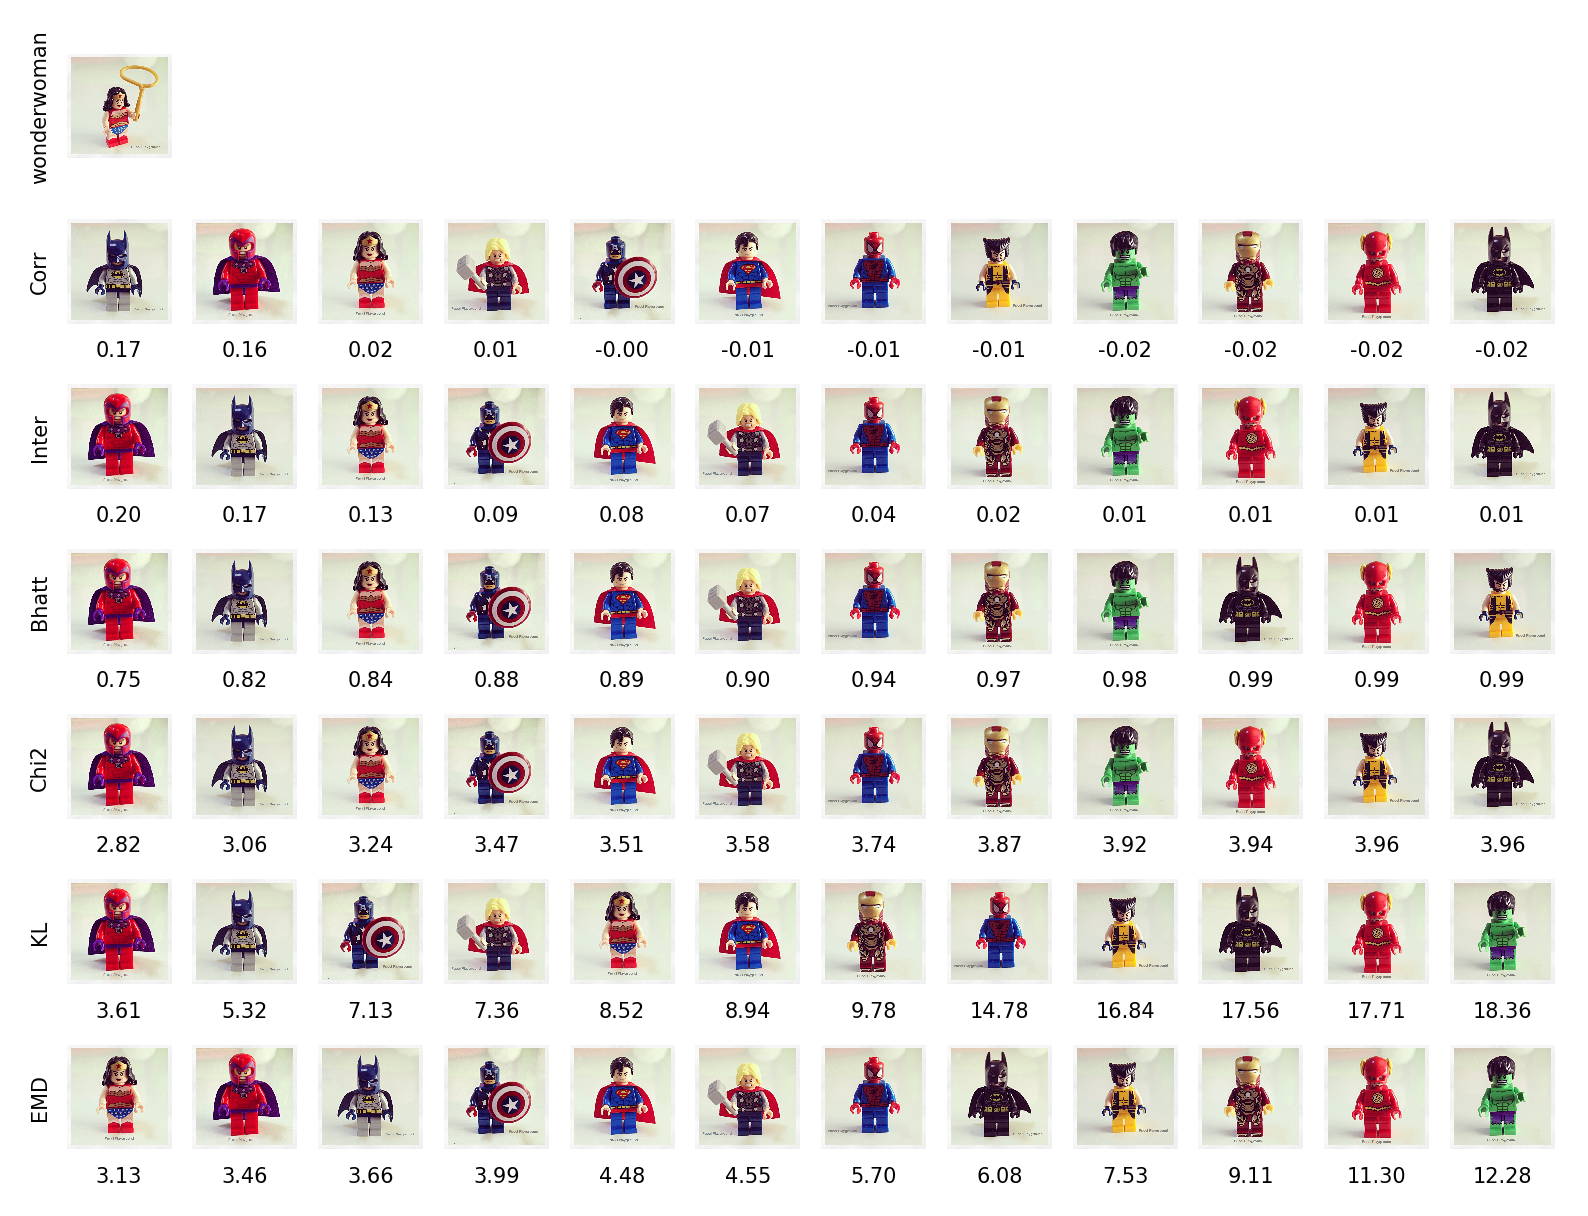
\includegraphics[width=0.9\textwidth]{cmpr_32_bins_lab_wonderwoman}
 \caption{Wonderwoman toy image retrieval example}
 \label{fig:wonderwoman_distances}
\end{figure}

\begin{figure}[!ht]
 \centering    
 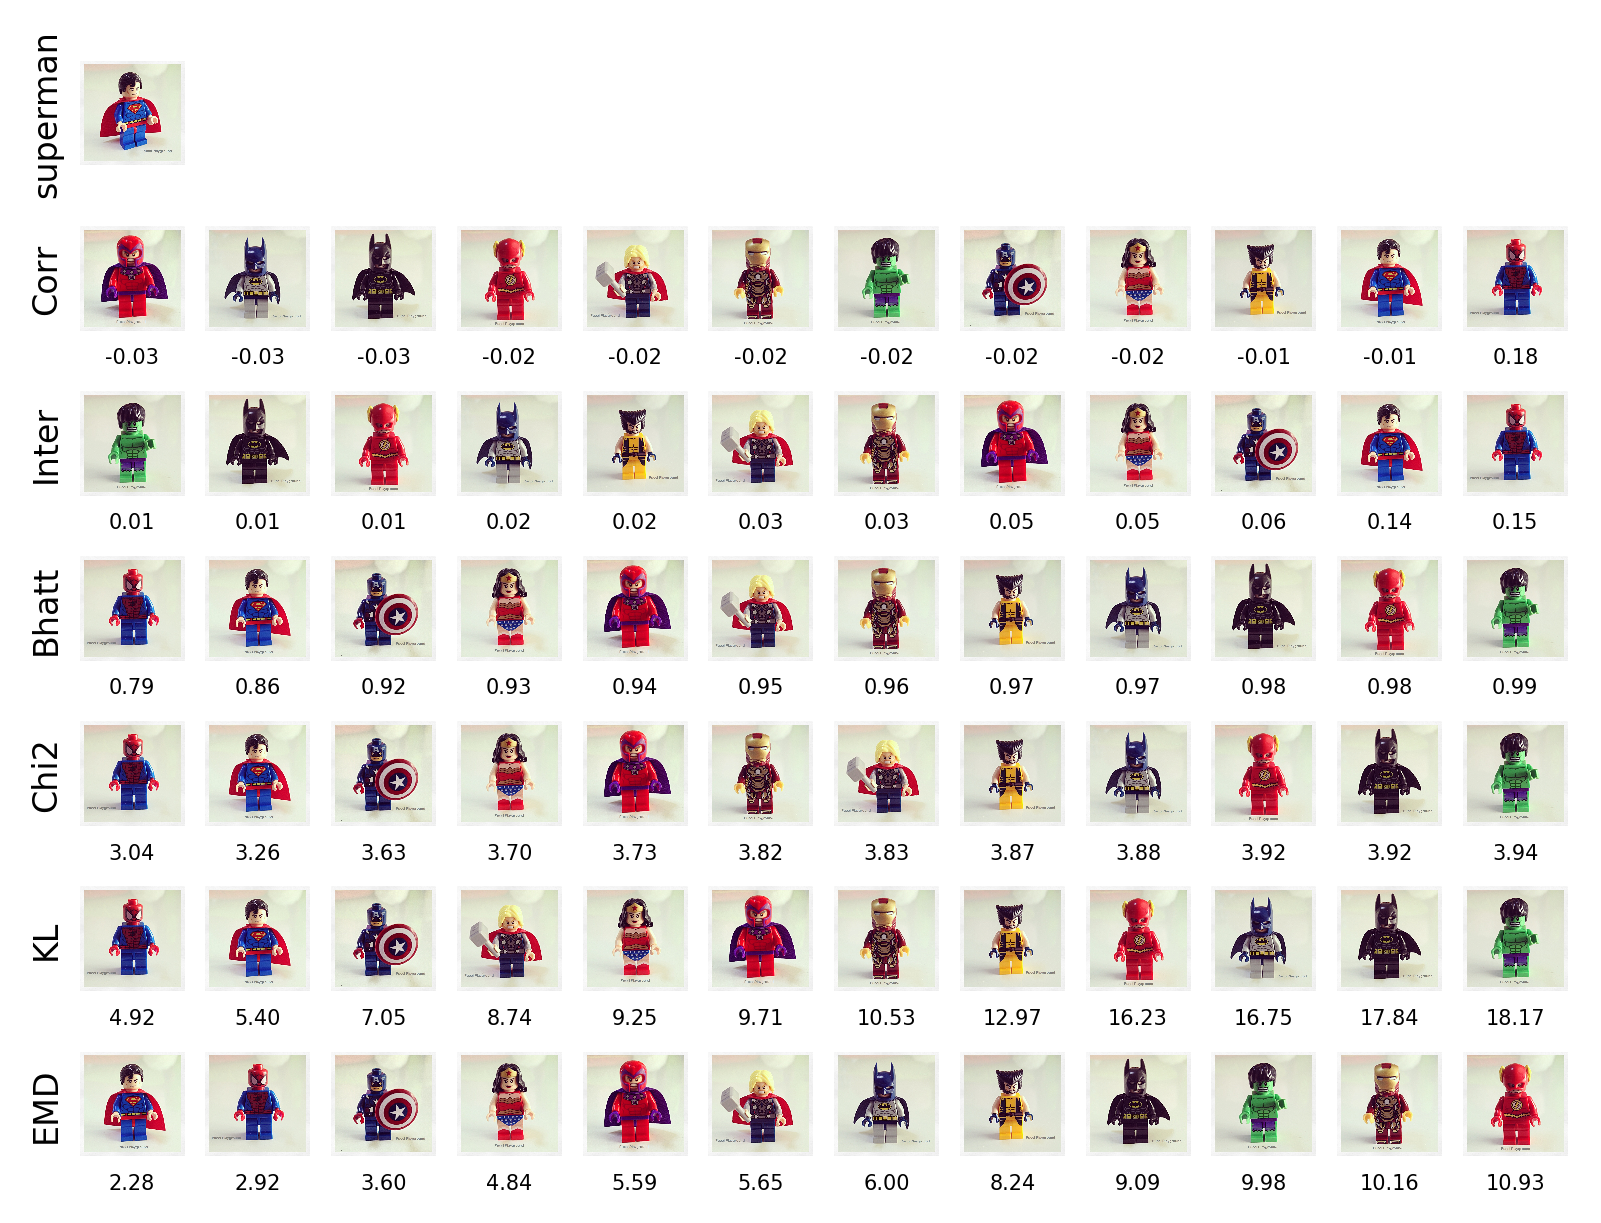
\includegraphics[width=0.9\textwidth]{cmpr_32_bins_lab_superman}
 \caption{Superman toy image retrieval example}
 \label{fig:superman_distances}
\end{figure}

\pagebreak
\subsubsection{Texture Projection Visual Evaluation}\label{sec:sm_mds}

The following images serve as a visual tool for the comparative evaluation of the different measures analyzed in this chapter. As we described in section \ref{subsec:mds}, the MDS technique allows to projecting the textures in a low dimensional space using the distances given by the similarity measures. This representation is carried out in a two-dimensional Euclidean space in our case. In the figures, we can notice that the MDS technique has problems representing the textures coherently when the input measures are not a metric, i.e., for the bin-to-bin measures. The axis in  Figs.\ \ref{fig:MDS_Inter} to \ref{fig:MDS_KL} do not correspond with the input space of the textures. According to the coarseness, we can speculate that there is a tendency to rank the textures in some arbitrary direction.

However, in the case of EMD, we can observe that since this measure uses a ground distance to calculate the similarity, we can define the cost matrix $\mathbf{C}_{ij} = c(x_i, y_j)$ of Eq. \ref{eq:optimal_work} to be the L1-distance as
\begin{eqnarray} 
 c(x_i, y_i) = d((\omega_i, \theta_i), (\omega_j, \theta_j))=\alpha|\Delta \omega| + |\Delta \theta| \label{eq:ground_distance}
\end{eqnarray}
where $|\Delta \omega| = \omega_i - \omega_j$, $\Delta \theta=min(|\theta_i-\theta_j|, \theta_{max} - |\theta_i-\theta_j|)$, and $\alpha$ is a constant that regulates the importance between the orientation and the coarseness of textures. In such a way that it represents the 2-d texture distributions into a log-polar space. We can distinguish this effect in Fig.\ \ref{fig:MDS_EMD} where we can see how the orientation and the frequency organize the textures into a log-polar coordinate space forming a circle. The texture orientation is represented along the circular axis; on the other hand, the texture frequency follows the axis going from the outside to the circle center. The lower frequency images remain at the edge of the circle, and those with high frequency (and low directionality) are grouped in the center. This behavior is not observed with any of the other measures and is reflected in the stress value of Fig.\ \ref{fig:stress}.

\begin{figure}[!ht]
 \centering    
 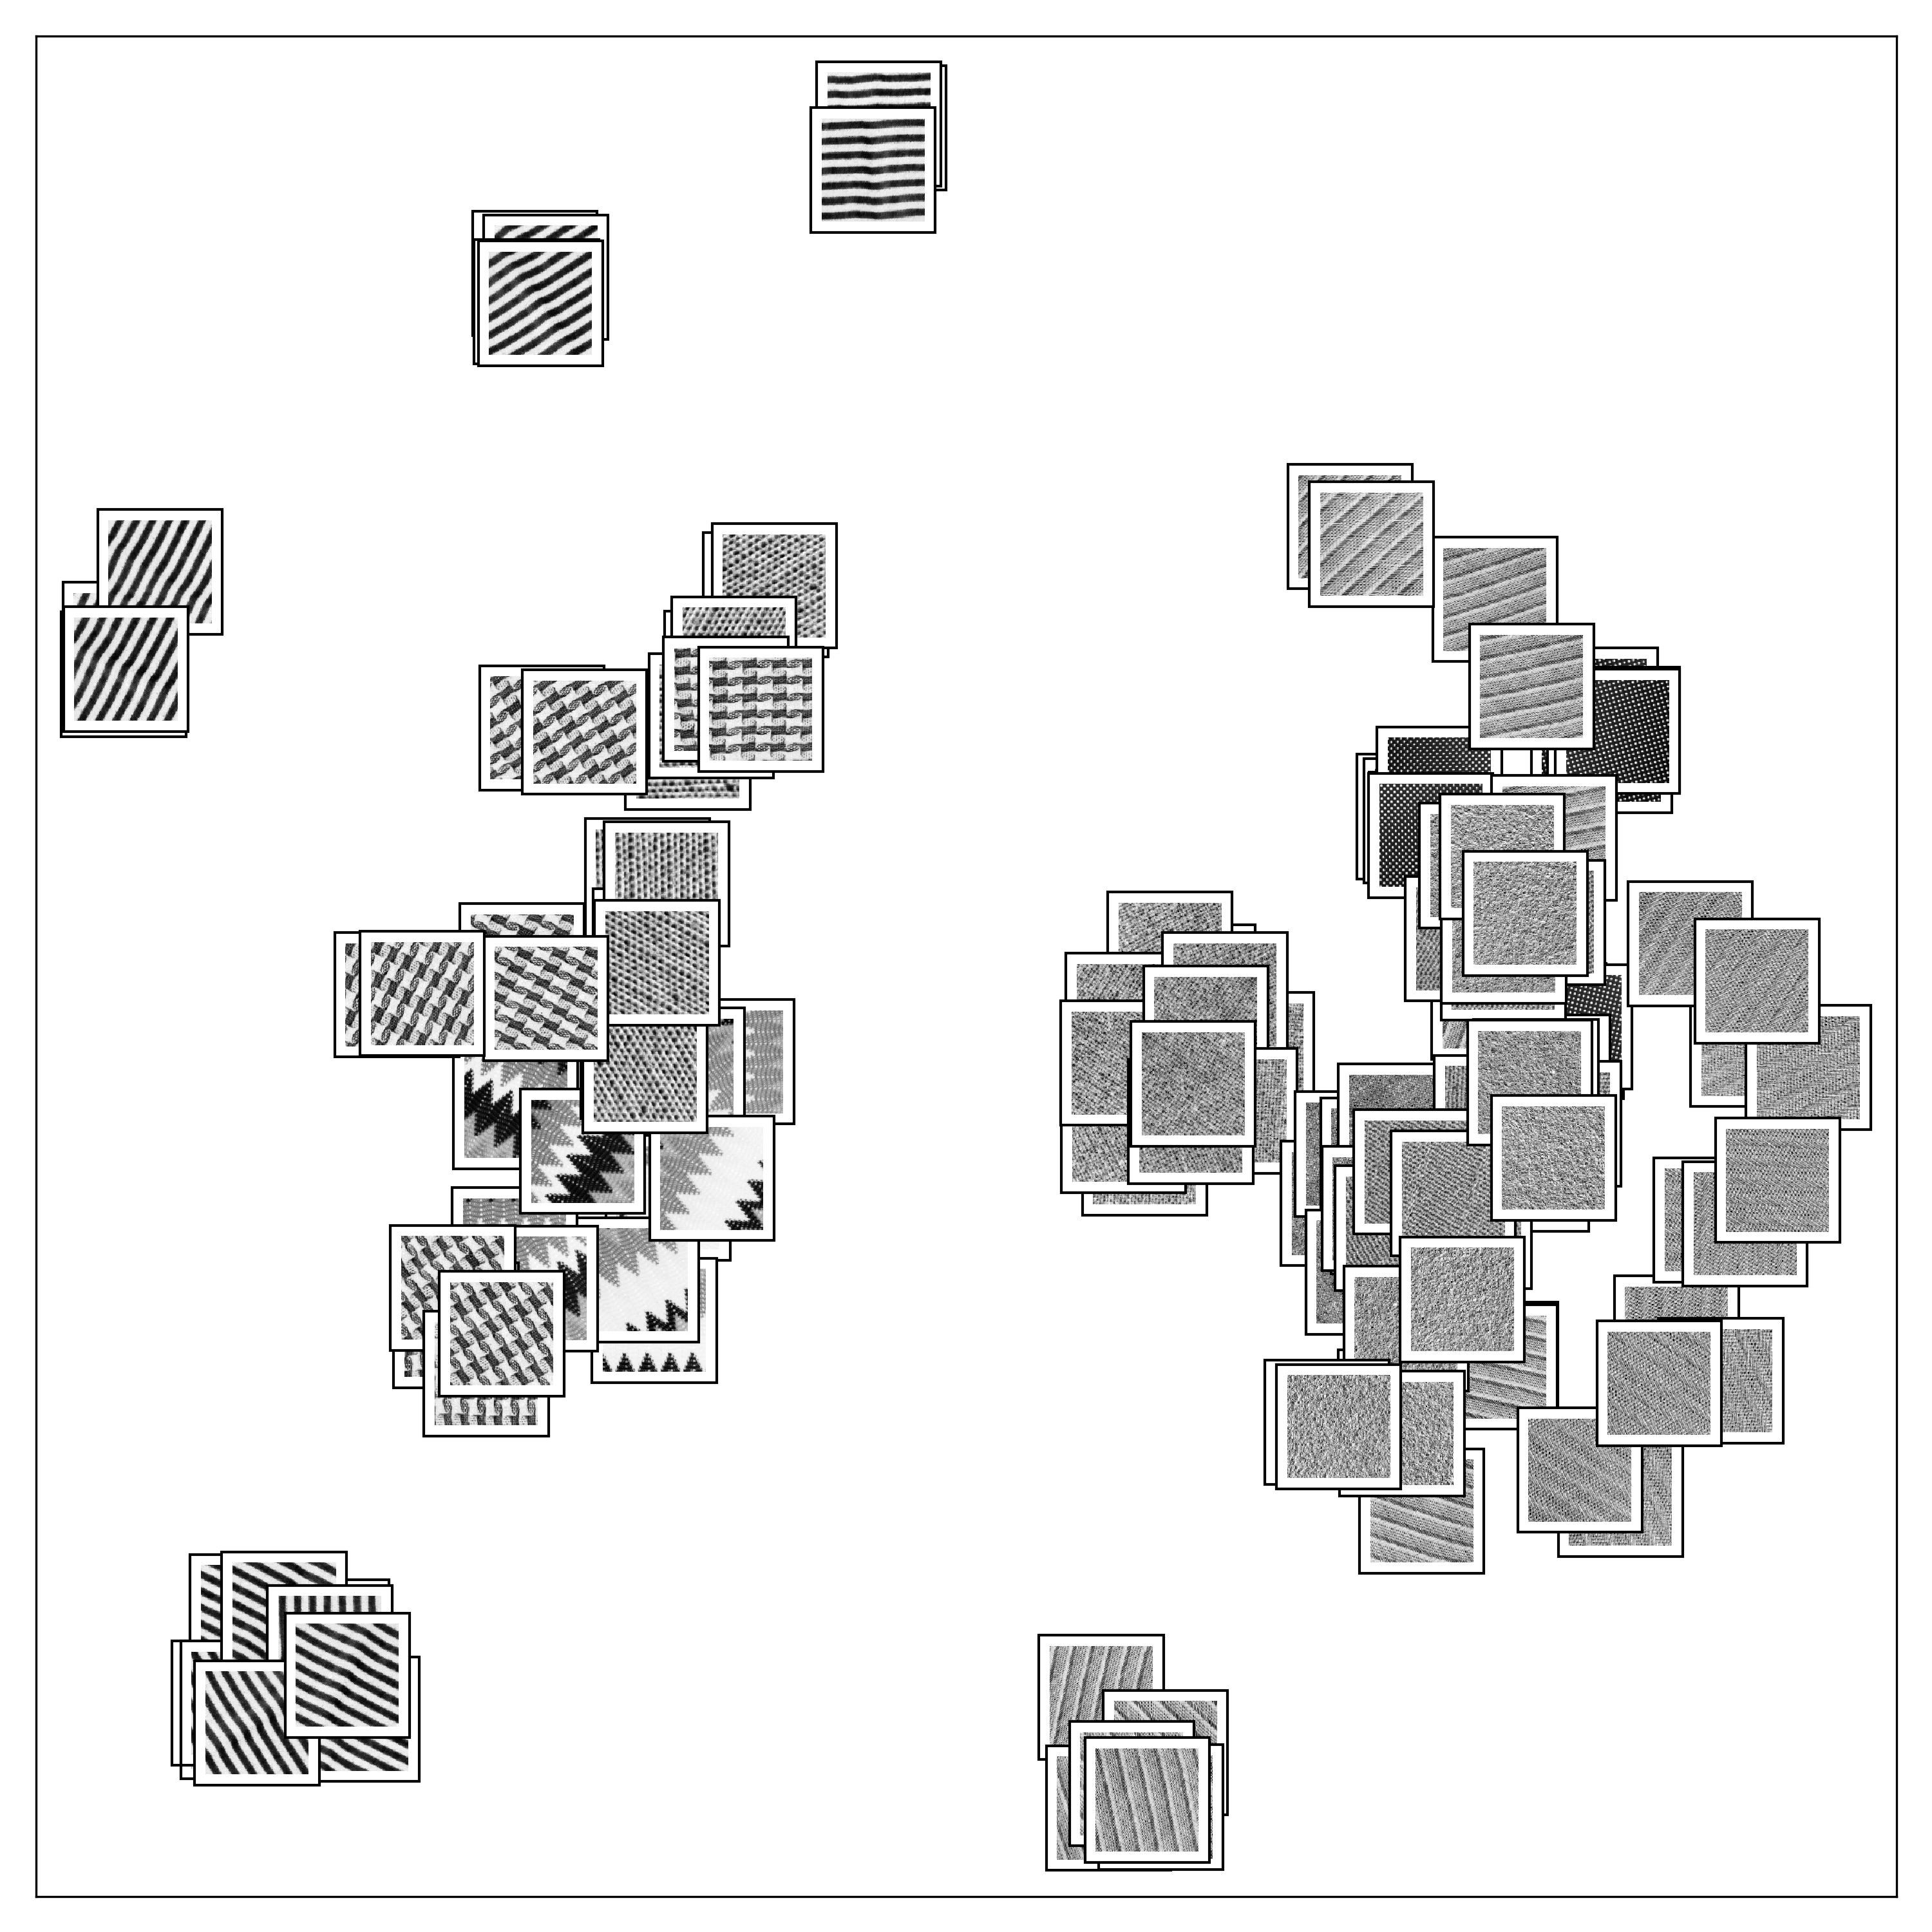
\includegraphics[width=0.7\textwidth]{MDS_Inter}
 \caption{MDS texture projection using the histogram intersection}
 \label{fig:MDS_Inter} 
\end{figure}

\begin{figure}[!ht]
 \centering    
 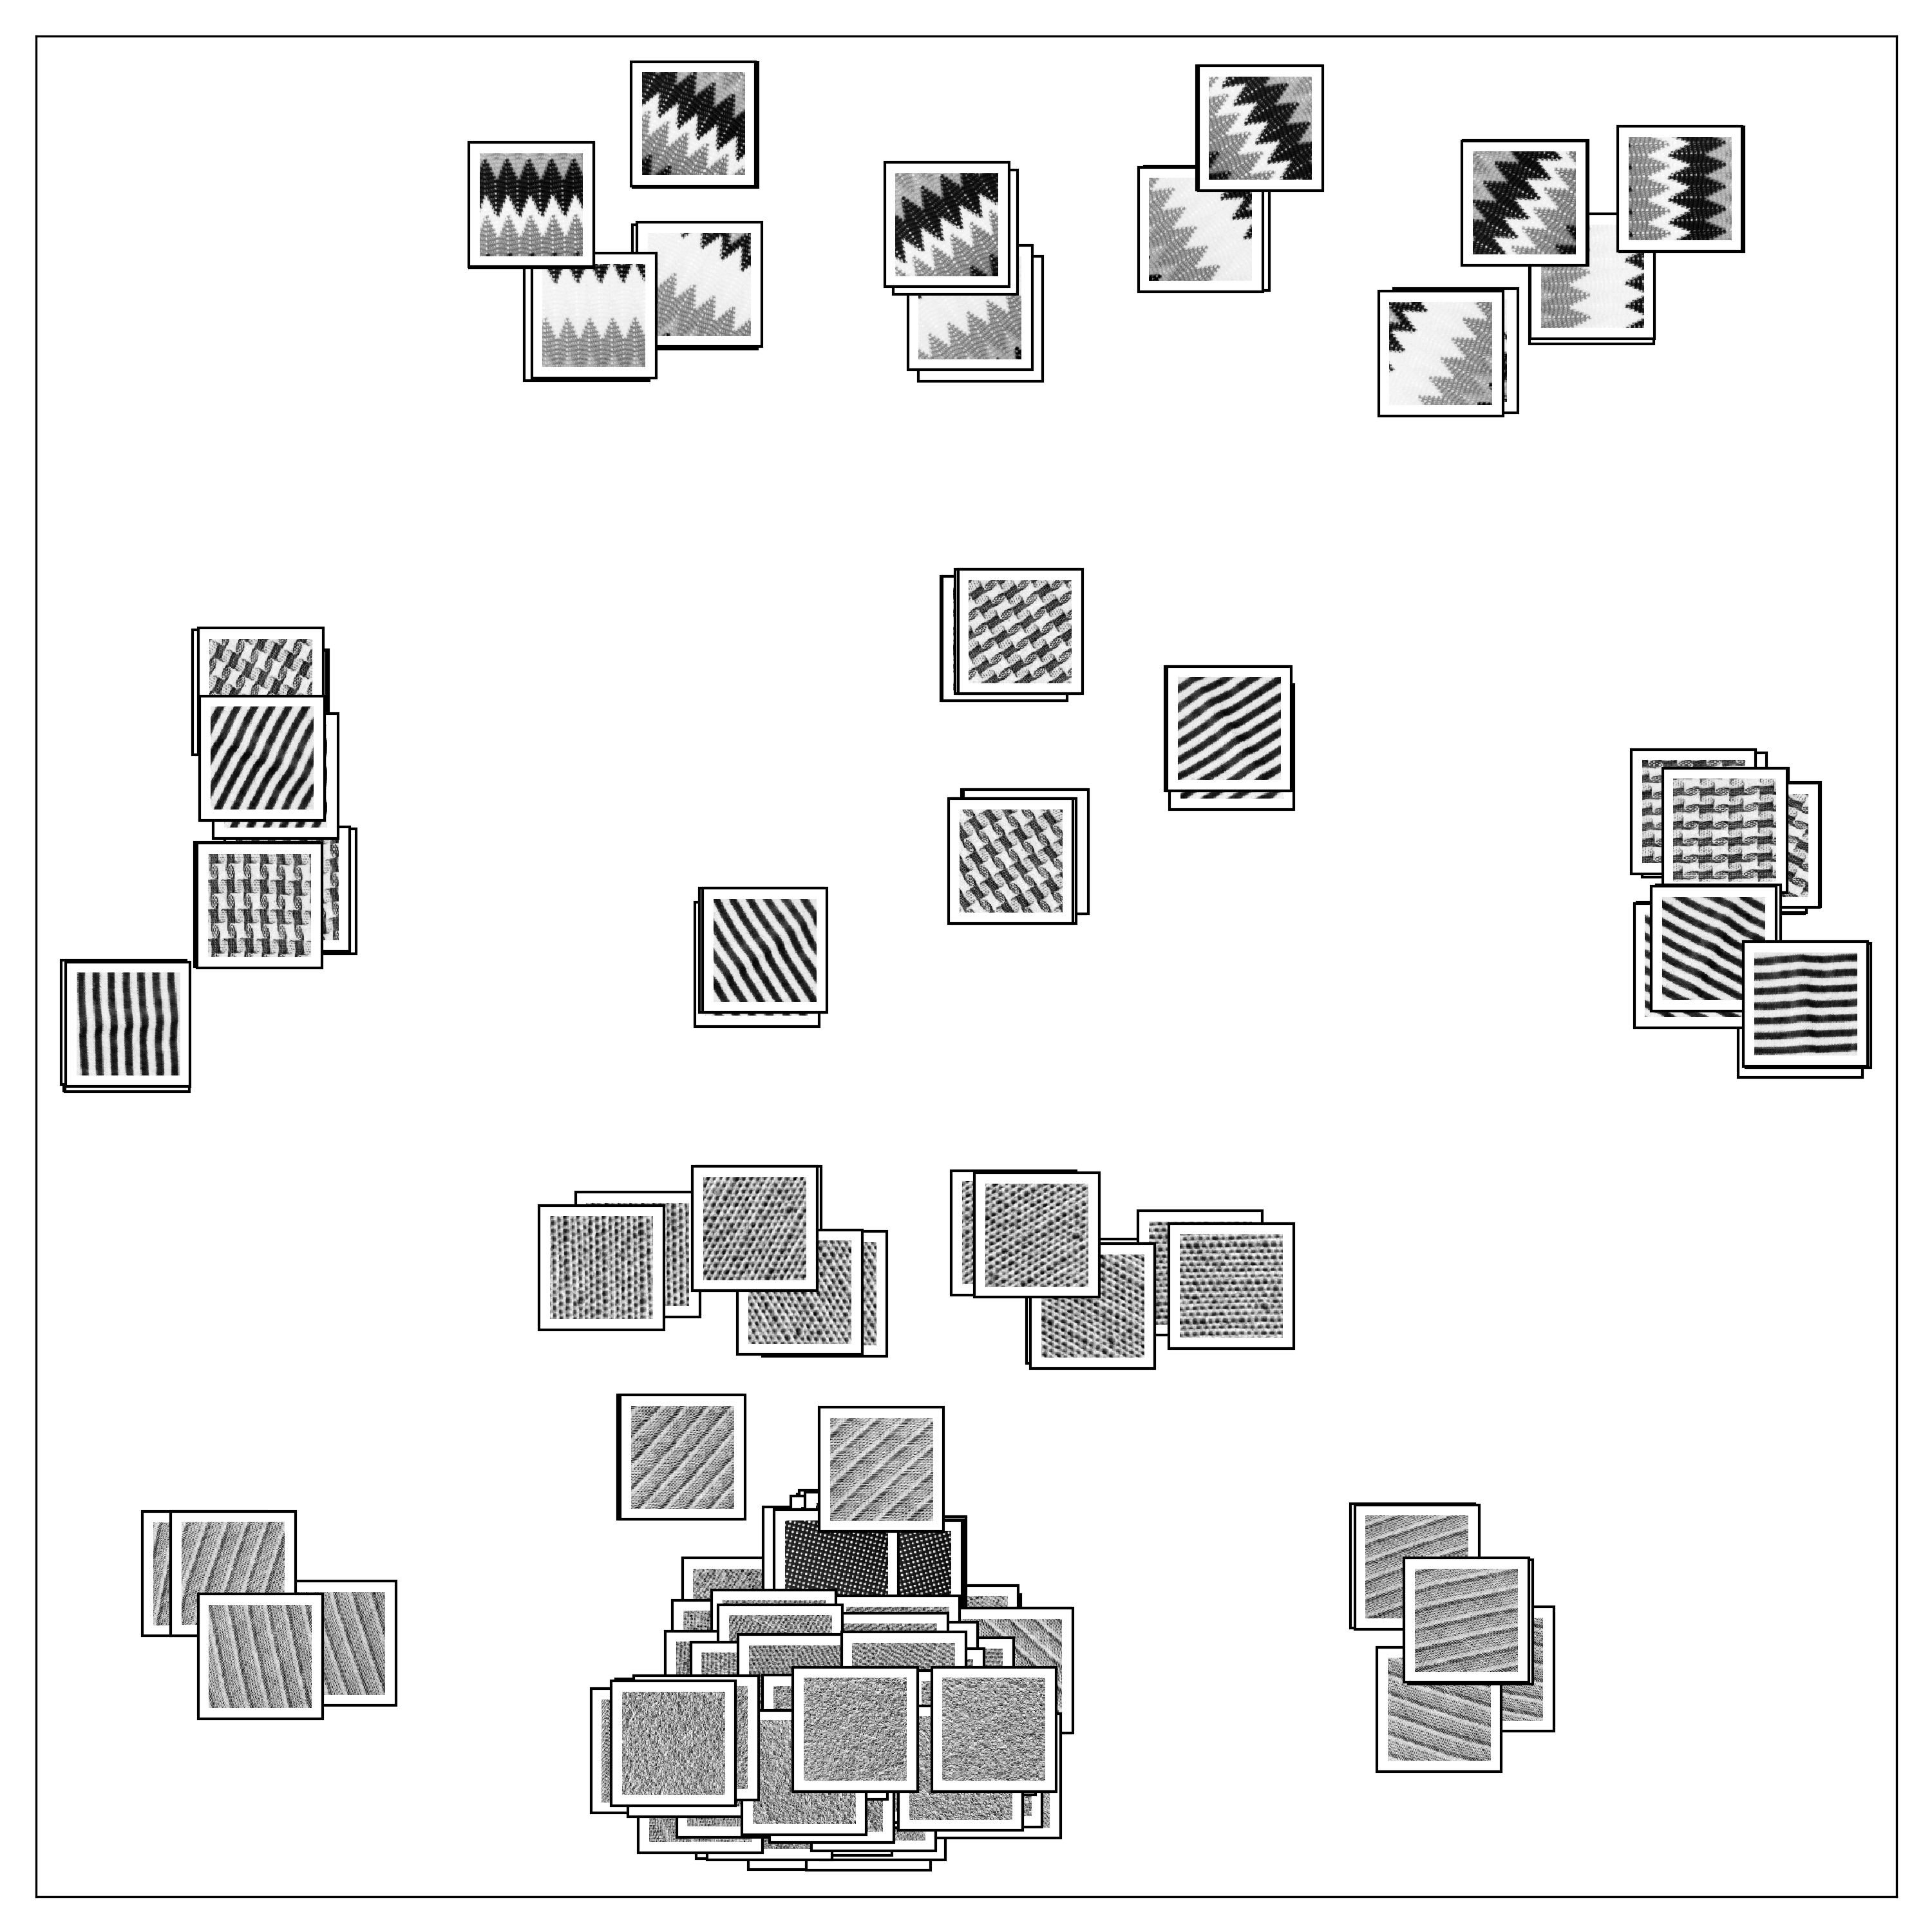
\includegraphics[width=0.7\textwidth]{MDS_Corr}
 \caption{MDS texture projection using the histogram correlation}
 \label{fig:MDS_Corr} 
\end{figure}

\begin{figure}[!ht]
 \centering    
 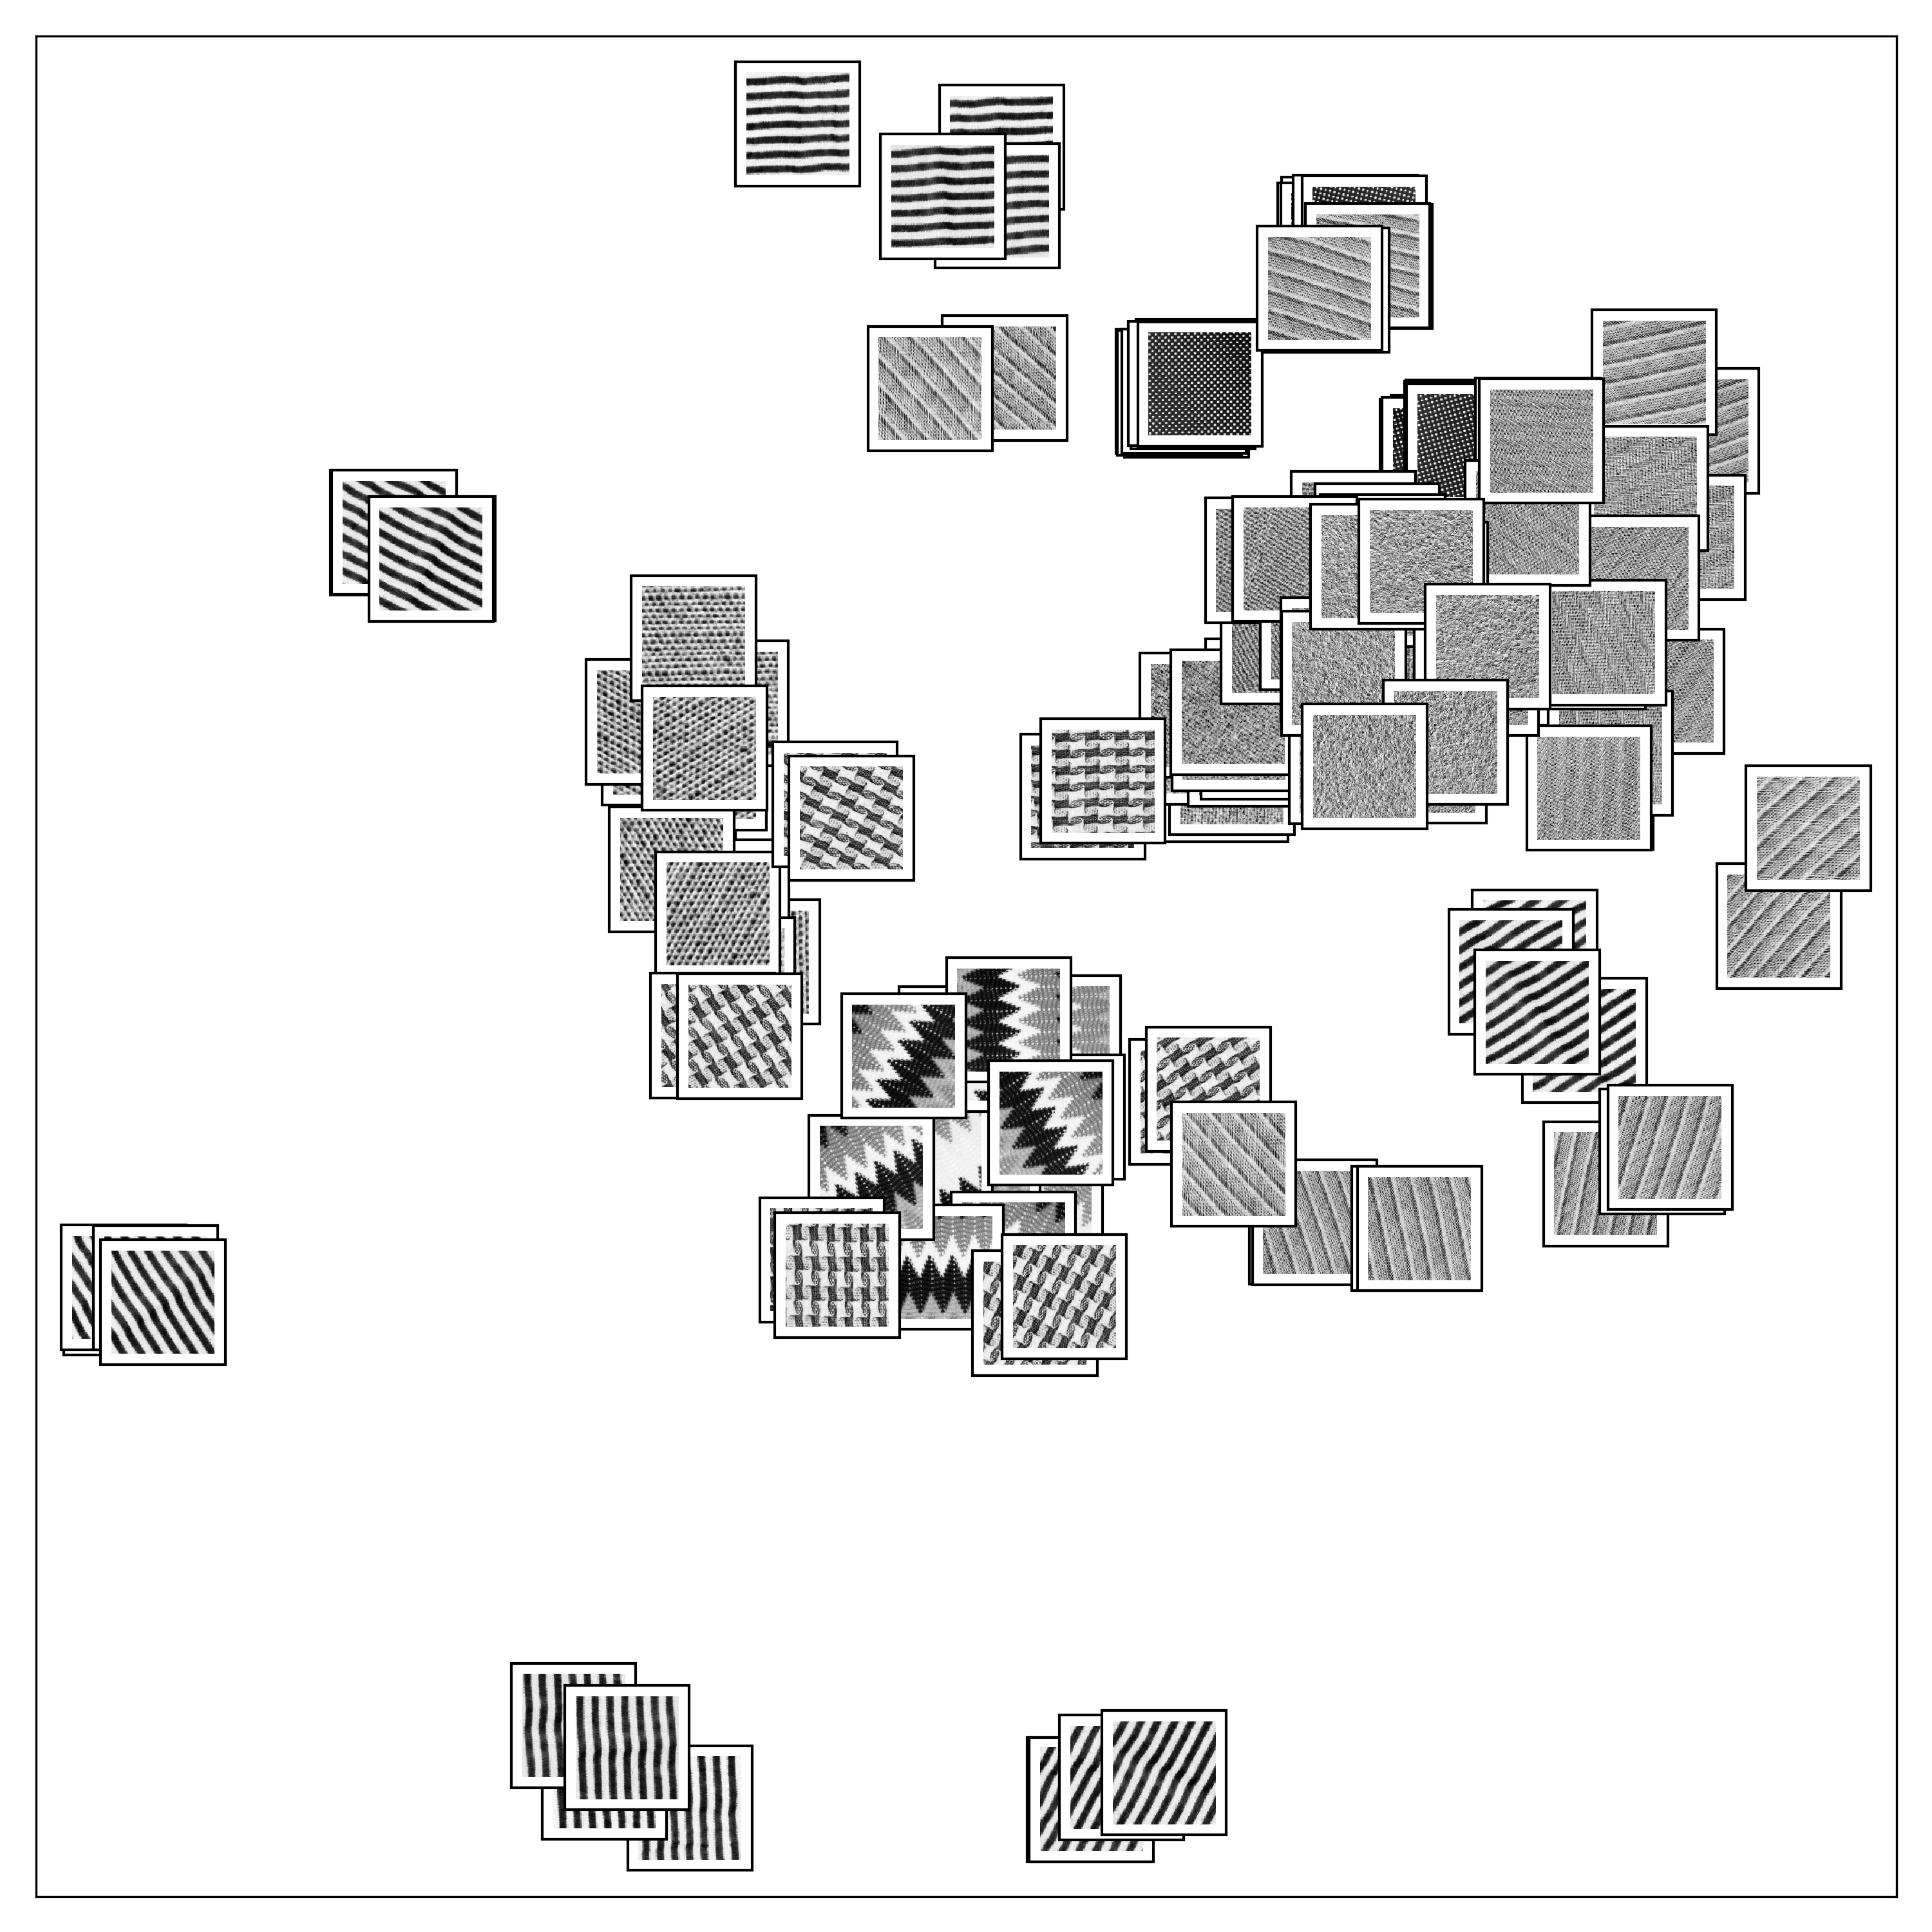
\includegraphics[width=0.7\textwidth]{MDS_Chi2}
 \caption{MDS texture projection using the $\chi^2$ statistic}
 \label{fig:MDS_Chi2} 
\end{figure}

\begin{figure}[!ht]
 \centering    
 \includegraphics[width=0.7\textwidth]{MDS_Bhatt}
 \caption{MDS texture projection using the Bhattacharyya distance}
 \label{fig:MDS_Bhatt} 
\end{figure}

\begin{figure}[!ht]
 \centering    
 \includegraphics[width=0.7\textwidth]{MDS_KL}
 \caption{MDS texture projection using the Kullback-Leibler divergence}
 \label{fig:MDS_KL} 
\end{figure}

\begin{figure}[!ht]
 \centering    
 \includegraphics[width=0.7\textwidth]{MDS_EMD2}
 \caption{MDS texture projection using the Earth Mover's Distance}
 \label{fig:MDS_EMD} 
\end{figure}

\section{Conclusion}\label{sec:conclusions}

In this chapter, we compare some of the few popular, bin-to-bin similarity measures with the EMD. We measure their performance in three tests: a one-dimensional analysis with synthetic distributions, two image classifiers (color and texture-based), and a visual projection using the MDS technique and the stress as the comparison value. The objective is to show that such measures highly used in the literature to develop complex tasks are not the best choice since they fail even in the most straightforward conditions. We illustrate that the EMD is a true metric \citep{Peyre.Cuturi:arXiv:2018} that naturally expresses dissimilarity between distributions.

\textbf{Results.}
The experiments of the previous sections show the superiority of the EMD to represent the similarity between distributions. First, the one-dimensional case shows how the bin-to-bin measures saturate (or fall to zero) as soon as the probabilities have an empty intersection (see Fig.\ \ref{fig:source_target_dist}). As for the image retrieval systems, we can see that by correctly choosing the feature image space and a good compression resolution of the distributions (LAB color space with 32 bins in the color-based system and the Gabor energy with eight bins in the texture-based system), the EMD performs the best classification result. However, this is not the case with the other measures because they are not a true distance. Representing the textures in the Euclidean space using the MDS technique shows another advantage of the EMD. The use of the ground distance $\textbf{C}$ in the optimal transport calculation makes it possible to transfer 2-d texture histograms to a logarithmic-polar space, making the stress value relatively low. 
%To see some examples of the color-based image retrieval system and the 2D texture projections, consult the file with supplementary material.

%\textbf{Furute Work.} Use of the metric for perceptual-based segmentation where the ground distance can be used to set specific weights for different measures like color, texture, intensity, contrast. This cannot be done without a ground distance.

\textbf{Notes about EMD computation complexity.}
We believe that EMD is a depreciated metric only because of its excessive calculation time. In the examples developed before, we calculate the EMD using the iterative process of linear programming. Despite this, the calculation is fast enough to develop the image classifier. In comparison with the first EMD algorithm \citep{Rubner.Tomasi.ea:IJCV:2000}, the computer processors' progress allows to use the same algorithm and be competitive with the bin-to-bin measures.
Moreover, a solution to the excessive complexity time and memory consumption is the regularized distances, also called Sinkhorn distances \citep{Cuturi:NIPS:2013}. This entropy-based regularization accelerates the computing time, giving a close approximation of the EMD. The regularization of distances allows for creating parallelizable algorithms.
